\documentclass[12pt, ngerman, a4paper, numbers=noenddot]{article} 
% --- Sprache & Encoding ---
\usepackage[utf8]{inputenc}
%\usepackage[T1]{fontenc}
%\usepackage[ngerman]{babel}
%\usepackage{lmodern}

\usepackage{fontspec}
\usepackage{polyglossia}
\setmainlanguage{german}
%\setmonofont{Latin Modern Mono} % oder eine andere Mono-Schriftart
\setmainfont{Latin Modern Roman}
\setmonofont{Fira Mono}


% --- Layout & Seitenränder ---
\usepackage[top=2cm, right=2cm, bottom=2cm, left=4cm]{geometry}
\usepackage{calc}
\usepackage{microtype}
\usepackage[htt]{hyphenat}


% --- Mathematik & Symbole ---
\usepackage{amsmath}
\usepackage{amssymb}


% --- Tabellen ---
\usepackage{array}
\usepackage{tabularx}          % Tabellen mit variabler Spaltenbreite
\usepackage{booktabs}

% --- Grafiken ---
\usepackage{graphicx}
\usepackage{float}

% --- Zeichnungen mit TikZ & Forest ---
\usepackage{tikz}
\usetikzlibrary{
	arrows.meta,        % für moderne Pfeile
	automata,
	shapes,
	calc,
	positioning,        % für node distance etc.
	quotes,
	graphs,             % TikZ Graph Library
	graphdrawing        % benötigt für layered layout etc.
}

% Falls versehentlich doppelt:
% \usetikzlibrary{shapes} ist schon enthalten, kann einmal entfernt werden

% Graph Drawing Libraries (nur mit LuaLaTeX oder XeLaTeX!)
\usegdlibrary{layered} % ← für layered layout
\usegdlibrary{force}   % ← falls du auch force-directed layouts nutzt

% Falls du forest nutzt:
\usepackage{forest}


% --- Farben & Listings (Code) ---
\usepackage{xcolor}
\usepackage{listings}

% Farbdefinitionen für Listings
\definecolor{backgray}{rgb}{0.95,0.95,0.95}
\definecolor{codegray}{rgb}{0.5,0.5,0.5}
\definecolor{codeblue}{rgb}{0.1,0.1,0.7}


% Eigene Sprache für Ordnerstrukturen
\lstdefinelanguage{folderstructure}{
	moredelim=**[is][\color{black}]{@}{@},
}

\lstdefinelanguage{json}{
	basicstyle=\ttfamily\footnotesize,
	numbers=left,
	numberstyle=\tiny\color{gray},
	stepnumber=1,
	numbersep=5pt,
	showstringspaces=false,
	breaklines=true,
	frame=single,
	backgroundcolor=\color{backgray},
	literate=
	*{0}{{{\color{codeblue}0}}}{1}
	{1}{{{\color{codeblue}1}}}{1}
	{2}{{{\color{codeblue}2}}}{1}
	{3}{{{\color{codeblue}3}}}{1}
	{4}{{{\color{codeblue}4}}}{1}
	{5}{{{\color{codeblue}5}}}{1}
	{6}{{{\color{codeblue}6}}}{1}
	{7}{{{\color{codeblue}7}}}{1}
	{8}{{{\color{codeblue}8}}}{1}
	{9}{{{\color{codeblue}9}}}{1}
	{:}{{{\color{black}:}}}{1}
	{,}{{{\color{black},}}}{1}
	{"}{{{\color{codeblue}"}}}{1},
}

\lstdefinelanguage{JavaScript}{
	keywords={break, case, catch, continue, debugger, default, delete, do, else, finally, for, function, if, in, instanceof, new, return, switch, this, throw, try, typeof, var, void, while, with, let, const, await, async},
	keywordstyle=\color{blue}\bfseries,
	ndkeywords={class, export, boolean, throw, implements, import, this},
	ndkeywordstyle=\color{darkgray}\bfseries,
	identifierstyle=\color{black},
	sensitive=false,
	comment=[l]{//},
	morecomment=[s]{/*}{*/},
	commentstyle=\color{codegray}\ttfamily,
	stringstyle=\color{codeblue},
	morestring=[b]',
	morestring=[b]",
}

\lstdefinelanguage{nginx}{
	morekeywords={
		server, location, listen, root, index, server_name,
		include, proxy_pass, try_files, rewrite, return, access_log, error_log
	},
	sensitive=false,
	morecomment=[l]{\#},
	morestring=[b]",
}

\lstdefinestyle{mystyle}{
	backgroundcolor=\color{backgray},
	commentstyle=\color{codegray}\ttfamily,
	keywordstyle=\color{blue}\bfseries,
	numberstyle=\tiny\color{gray},
	stringstyle=\color{codeblue},
	basicstyle=\ttfamily\footnotesize,
	breaklines=true,
	captionpos=b,
	keepspaces=true,
	numbers=left,
	numbersep=5pt,
	showspaces=false,
	showstringspaces=false,
	showtabs=false,
	tabsize=2,
}

\lstset{style=mystyle}


% --- Bibliographie ---
\usepackage[backend=biber, style=ieee, url=true]{biblatex}
\addbibresource{./Bibliothek.bib}
\usepackage{csquotes}

% --- Schriftart für Monospace ---
%\usepackage{bera} % schöne Mono-Schrift optional
%\setmonofont{Fira Mono} % oder Latin Modern Mono, oder eine Systemschrift wie Consolas
%\setmonofont{Latin Modern Mono}

% --- Zeilenabstand ---
\usepackage{setspace}
\onehalfspacing

% --- Kopfzeile ---
\usepackage[automark]{scrlayer-scrpage}
\pagestyle{scrheadings}
\clearscrheadings
\ihead{}
%\ihead[\rightmark]{\pagemark}
\chead{}
%\chead{}{}
\ohead{\pagemark}
%\ohead[\pagemark]{\rightmark}

% --- Hyperlinks ---

\PassOptionsToPackage{hyphens}{url}
\usepackage{hyperref}
\usepackage{xurl}



% --- Sonstiges ---
\usepackage[official]{eurosym}
\usepackage{lastpage}
\usepackage{etoolbox}
\usepackage{listings}


\usepackage[toc=false]{glossaries-extra}


% Kategorien definieren
\newglossary[flg]{frontend}{fnd}{fnt}{Frontend-Technologien}
\newglossary[bkg]{backend}{bdg}{bdt}{Backend-Technologien und Java}
\newglossary[dbg]{db}{ddg}{ddt}{Datenbanken und Indizes}
\newglossary[srg]{server}{sdg}{sdt}{Server und Infrastruktur}
%\newglossary[spg]{storage2}{spg}{spt}{Storage22}
\newglossary[otg]{misc}{mdg}{mdt}{Speichertechnologien}

% Frontend-Technologien
\newglossaryentry{vuejs}{
	name=Vue.js,
	description={Ein progressives JavaScript-Framework zur Erstellung interaktiver Benutzeroberflächen. Es ähnelt AngularJS und React, ist aber besonders leichtgewichtig und flexibel.},
	type=frontend
}
\newglossaryentry{vue3}{
	name=Vue 3,
	description={Die aktuelle Hauptversion von Vue.js, die neue Features wie die Composition API für bessere Code-Organisation und höhere Leistung bietet.},
	type=frontend
}
\newglossaryentry{vuecli}{
	name=Vue CLI,
	description={Ein Kommandozeilen-Werkzeug zum schnellen Erstellen und Verwalten von Vue-Projekten mit integrierten Build-Tools und Plugins.},
	type=frontend
}
\newglossaryentry{dom}{
	name=DOM,
	description={Das Document Object Model ist eine standardisierte, baumartige Darstellung von HTML- und XML-Dokumenten, die es Skriptsprachen wie JavaScript ermöglicht, Inhalte, Struktur und Stil einer Webseite dynamisch zu verändern.},
	type=frontend
}
\newglossaryentry{framework}{
	name=Framework,
	description={Eine wiederverwendbare Softwarestruktur, die als Gerüst für die Entwicklung von Anwendungen dient. Frameworks stellen vorgefertigte Funktionen und Konventionen bereit, um typische Programmieraufgaben zu vereinfachen und zu standardisieren. Beispiele sind \emph{Spring Boot} für Java oder \emph{Vue.js} für das Web-Frontend.},
	type=frontend
}
\newglossaryentry{sfc}{
	name=Single-File Component (SFC),
	description={Dateien, die Template, Logik und Styles in einer einzigen .vue-Datei bündeln und so modularen und übersichtlichen Code ermöglichen.},
	type=frontend
}
\newglossaryentry{compositionapi}{
	name=Composition API,
	description={Ein modernes Programmiermodell in Vue 3 zur besseren Strukturierung von Komponentenlogik, besonders nützlich für komplexe Anwendungen.},
	type=frontend
}
\newglossaryentry{spa}{
	name=Single-Page Application (SPA),
	description={Webanwendungen, die in einer einzelnen HTML-Seite laufen und Inhalte dynamisch nachladen, um schnelle und flüssige Nutzererlebnisse zu ermöglichen.},
	type=frontend
}
\newglossaryentry{axios}{
	name=Axios,
	description={Eine JavaScript-Bibliothek zum einfachen Senden von HTTP-Anfragen, besonders für die Kommunikation mit REST-APIs.},
	type=frontend
}
\newglossaryentry{cors}{
	name=CORS (Cross-Origin Resource Sharing),
	description={Ein Sicherheitsmechanismus, der steuert, welche Ressourcen von einer Webdomain aus auf eine andere zugreifen dürfen.},
	type=frontend
}
\newglossaryentry{preflight}{
	name=Preflight-Anfrage,
	description={Eine automatische OPTIONS-Anfrage des Browsers zur Überprüfung von CORS-Richtlinien vor der eigentlichen HTTP-Anfrage.},
	type=frontend
}
\newglossaryentry{historyapi}{
	name=History API,
	description={Browser-API zur Manipulation des Verlaufs und der URL, wichtig für Navigation in SPAs ohne Seitenreload.},
	type=frontend
}

% Backend-Technologien & Java
\newglossaryentry{backend}{
	name=Backend,
	description={Der Teil einer Anwendung, der serverseitig Daten verarbeitet, Logik ausführt und Schnittstellen zu Datenbanken bereitstellt.},
	type=backend
}
\newglossaryentry{api}{
	name=API (Application Programming Interface),
	description={Eine Schnittstelle, die es ermöglicht, dass verschiedene Softwarekomponenten miteinander kommunizieren. APIs definieren, wie Funktionen, Daten und Dienste von einem Programm für andere Programme zugänglich gemacht werden. Beispiele in diesem Projekt sind die \emph{FFM API} zur Anbindung nativer Funktionen und die \emph{Enigma-API} als REST-Schnittstelle zur Enigma-Verschlüsselung.},
	type=backend
}
\newglossaryentry{springboot}{
	name=Spring Boot,
	description={Ein Framework zur Entwicklung von Java-Anwendungen, das auf dem Spring-Framework aufbaut. Es ermöglicht durch Konventionen und automatische Konfiguration eine schnelle Einrichtung von produktionsreifen Webanwendungen. Spring Boot unterstützt die Entwicklung von REST-APIs, Validierung (z.\,B. mit \lstinline|javax.validation|) sowie Dependency Injection und bietet umfangreiche Middleware-Integration.},
	type=backend
}
\newglossaryentry{rest}{
	name=REST (Representational State Transfer),
	description={Ein Architekturstil für Webservices, der auf HTTP-Methoden (GET, POST, PUT, DELETE) basiert. REST definiert Prinzipien wie zustandslose Kommunikation, klare Ressourcennamen (URLs) und standardisierte Operationen. APIs, die diese Prinzipien befolgen, werden als \emph{RESTful} bezeichnet und ermöglichen einfache, skalierbare und leicht verständliche Schnittstellen.},
	type=backend
}
\newglossaryentry{restful}{
	name=RESTful HTTP-API,
	description={Eine Web-API, welche die Prinzipien von REST nutzt, um Ressourcen über HTTP-Methoden zugänglich zu machen.},
	type=backend
}
\newglossaryentry{dto}{
	name=DTO (Data Transfer Object),
	description={Einfache Datenstruktur zur Übertragung von Daten zwischen verschiedenen Schichten einer Anwendung, z.\,B.\ zwischen Controller und Service.},
	type=backend
}
\newglossaryentry{responseentity}{
	name=ResponseEntity,
	description={Klasse zur flexiblen Modellierung von HTTP-Antworten, inklusive Statuscode und Headern.},
	type=backend
}
\newglossaryentry{service}{
	name=Service-Schicht,
	description={Softwarearchitektur-Schicht, die Geschäftslogik kapselt und von Controllern genutzt wird.},
	type=backend
}
\newglossaryentry{jdbc}{
	name=JDBC (Java Database Connectivity),
	description={Standard-API in Java zur Kommunikation mit relationalen Datenbanken.},
	type=backend
}
\newglossaryentry{hibernate}{
	name=Hibernate,
	description={Java-Framework für Objekt-Relationale Abbildung (ORM), das SQL-Komplexität reduziert.},
	type=backend
}
\newglossaryentry{ffmapi}{
	name=Java Foreign Function und Memory API (FFM API),
	description={Eine moderne Java-API zur effizienten und sicheren Anbindung nativer Bibliotheken (z.\,B. in C). Sie ermöglicht direkten Zugriff auf native Funktionen und Speicher, als Nachfolger des älteren JNI-Mechanismus, mit einfacherem und performanterem Code.},
	type=backend
}
\newglossaryentry{jni}{
	name=Java Native Interface (JNI),
	description={Ältere Schnittstelle zum Aufruf nativer Bibliotheken aus Java, komplexer als FFM API.},
	type=backend
}
\newglossaryentry{nativefunc}{
	name=Native Funktion,
	description={Funktion, die außerhalb der Java Virtual Machine (JVM) in einer anderen Programmiersprache wie C oder C++ implementiert ist und über Schnittstellen wie JNI oder die Foreign Function \& Memory API (FFM API) von Java aufgerufen wird.},
	type=backend
}

% Datenbanken & Indizes
\newglossaryentry{postgresql}{
	name=PostgreSQL,
	description={Leistungsstarkes, objektrelationales Open-Source-Datenbank\-system mit umfangreichen Managementfunktionen.},
	type=db
}
\newglossaryentry{primarykey}{
	name=Primärschlüssel,
	description={Ein eindeutiges Attribut oder eine Attributkombination, die jeden Datensatz in einer Tabelle eindeutig identifiziert. Primärschlüssel sind fundamental für Datenintegrität und die Herstellung von Beziehungen in relationalen Datenbanken. Besteht der Primärschlüssel aus mehreren Attributen, so spricht man von einem zusammengesetzten Primärschlüssel.},
	type=db
}
\newglossaryentry{foreignkey}{
	name=Fremdschlüssel,
	description={Ein Attribut, das auf einen Primärschlüssel einer anderen Tabelle verweist und somit eine Beziehung zwischen Tabellen definiert. Fremdschlüssel sorgen für referenzielle Integrität und verhindern inkonsistente Daten.},
	type=db
}
\newglossaryentry{normalization}{
	name=Normalisierung,
	description={Ein Verfahren zur Strukturierung von Datenbanken, das Redundanzen vermeidet und die Datenintegrität durch die Einhaltung von Normalformen (z.\,B. dritte Normalform, 3NF) sicherstellt. Normalisierung verbessert die Wartbarkeit und Konsistenz der Daten.},
	type=db
}
\newglossaryentry{ginindex}{
	name=GIN-Index (Generalized Inverted Index),
	description={Ein spezieller Index in PostgreSQL, der schnelle Volltextsuche und Abfragen auf komplexen Datentypen wie Arrays und JSONB ermöglicht. Er optimiert Suchanfragen durch Invertierung der Datenstruktur.},
	type=db
}
\newglossaryentry{containmentoperator}{
	name=Containment Operator ({@>}),
	description={Operator zur Abfrage, ob ein Array oder JSON ein bestimmtes Element enthält.},
	type=db
}
\newglossaryentry{pagination}{
	name=Pagination,
	description={Die Unterteilung großer Datenmengen in überschaubare Seiten (Pages) zur Verbesserung der Performance und Nutzerfreundlichkeit. Pagination reduziert die Netzwerklast und die Ladezeiten beim Abrufen von Datensätzen aus der Datenbank.},
	type=db
}

\newglossaryentry{planner}{
	name=Query-Planner,
	description={Komponente einer Datenbank, die entscheidet, wie eine Abfrage ausgeführt wird, um sie möglichst effizient zu machen.},
	type=db
}

% Server & Infrastruktur
\newglossaryentry{nginx}{
	name=nginx,
	description={Beliebter, performanter Webserver und Reverse-Proxy.},
	type=server
}
\newglossaryentry{reverseproxy}{
	name=Reverse-Proxy,
	description={Server, der Anfragen an Backend-Server weiterleitet, oft für Lastverteilung und Sicherheit genutzt.},
	type=server
}
\newglossaryentry{systemd}{
	name=systemd-Dienst,
	description={Linux-Manager für Hintergrundprozesse (Dienste).},
	type=server
}
\newglossaryentry{httpcompression}{
	name=HTTP-Kompression,
	description={Verfahren zur Reduktion der Größe von HTTP-Antworten zur Beschleunigung der Datenübertragung.},
	type=server
}
\newglossaryentry{caching}{
	name=Caching,
	description={Zwischenspeicherung häufig genutzter Daten, um Ladezeiten und Serverlast zu verringern.},
	type=server
}

% Speicher & Programmierung
\newglossaryentry{memorysegment}{
	name=MemorySegment,
	description={Speicherbereich in der Java FFM API für sicheren Zugriff auf nativen Speicher.},
	type=misc
}
\newglossaryentry{methodhandle}{
	name=MethodHandle,
	description={Java-Objekt zur dynamischen Methodenreferenzierung.},
	type=misc
}
\newglossaryentry{functiondescriptor}{
	name=FunctionDescriptor,
	description={Beschreibung der Signatur nativer Funktionen für die FFM API.},
	type=misc
}
\newglossaryentry{memorylayout}{
	name=Speicher-Layout (MemoryLayout),
	description={Anordnung von Daten im Speicher für Kompatibilität mit nativen Bibliotheken.},
	type=misc
}
\newglossaryentry{speicheralignment}{
	name=Speicher-Alignment,
	description={Ausrichtung von Daten im Speicher nach bestimmten Grenzen für Performance und Kompatibilität.},
	type=misc
}

% Sonstiges

\makeglossaries



%-------------- Ende allgemeine Angaben -----------------------------
\begin{document}

%-------------- Beginn Titelseite -----------------------------------
\hypersetup{pageanchor=false}
\thispagestyle{empty}
%\includegraphics[height=2.4cm, trim=1.2cm 1.2cm 1.2cm 1.2cm]{UniLogo.jpg}
%\vspace{2.4cm}
\vspace{1cm}
%\begin{center}
\begin{flushleft}
%RWU–University of Applied Sciences\\
\begin{figure}[H]
	
\includegraphics[width=0.3\textwidth]{bilder/RWU.pdf}
\end{figure}
\vspace{4cm}
%{\huge Bachelorarbeit} \\
{\fontsize{50pt}{42pt}\selectfont \textbf{Bachelorthesis}} \\



\vspace{2cm}
{\Huge Entwicklung einer Webseite zur Veranschaulichung der Ver- und Entschlüsselungsmethoden der Enigma.} \\

%\vspace{3cm}
%Prüfer: Prof. Dipl.-Math. Ekkehard Löhmann \\
%{Prof. Dr.-Ing. Thorsten Weiss} \\
%\end{center}

\vspace{3cm}

\begin{tabular}{@{}l l@{}}
	Vorgelegt von: & Tobias Steidle \\
	wohnhaft in: & Dreiländerring 44, 88212 Ravensburg \\
	geboren am: & 18.10.1992 \\
	geboren in: & Weingarten \\
	& \\ % Leerzeile
	\multicolumn{2}{@{}l}{Hochschule Ravensburg-Weingarten} \\
	Fakultät: & Elektrotechnik und Informatik \\
	Studiengang: & Informatik/Elektrotechnik PLUS \\
	& \\
	1. Prüfer: & Prof. Dipl.-Math. Ekkehard Löhmann \\
	2. Prüfer: & Prof. Dr.-Ing. Thorsten Weiss \\
	& \\
	Ausgabedatum: & 11.12.2024 \\
	Abgabedatum: & 08.07.2025 \\
\end{tabular}

\end{flushleft}



%-------------- Ende Titelseite -------------------------------------


%-------------- Inhaltsverzeichnis
\newpage
\hypersetup{pageanchor=true}
\pagenumbering{Roman}
\renewcommand{\thepage}{\Roman{page}}


%-------------- Eidesstattliche Erklärung ----------------------------
\newpage
\section*{Eidesstattliche Erklärung}
Ich versichere an Eides statt, dass ich die vorstehende Arbeit selbständig und ohne fremde Hilfe angefertigt und mich anderer als der im beigefügten Verzeichnis angegebenen Hilfsmittel nicht bedient habe. Alle Stellen, die wörtlich oder sinngemäß aus Veröffentlichungen übernommen wurden, sind als solche kenntlich gemacht. Alle Internetquellen sind der Arbeit beigefügt. Des Weiteren versichere ich, dass ich die Arbeit vorher nicht in einem anderen Prüfungsverfahren eingereicht habe und dass die eingereichte schriftliche Fassung der auf dem elektronischen Speichermedium entspricht.\\
\begin{flushleft}
	Ravensburg, 07.07.2025
	\ \\
	\ \\
	\ \\
	\ \\
	\ \\
	Tobias Steidle
\end{flushleft}

\newpage
\tableofcontents{}

%%-------------- Abbildungsverzeichnis 
%\newpage
%\cleardoublepage\phantomsection
%\addcontentsline{toc}{section}{Abbildungsverzeichnis}
%\listoffigures
%
%
%%-------------- Tabellenverzeichnis
%\newpage
%\cleardoublepage\phantomsection
%\addcontentsline{toc}{section}{Tabellenverzeichnis}
%\listoftables
%
%
%%-------------- Abkürzungsverzeichnis
%\newpage
%\cleardoublepage\phantomsection
%\addcontentsline{toc}{section}{Abkürzungsverzeichnis}
%\section*{Abkürzungsverzeichnis}
%
%
%%-------------- Symbolverzeichnis
%\newpage
%\cleardoublepage\phantomsection
%\addcontentsline{toc}{section}{Symbolverzeichnis}
%\section*{Symbolverzeichnis}
%
%
%

\newpage
\pagenumbering{arabic}
\renewcommand{\thepage}{\arabic{page}}



	



\newpage

\glsaddall

\section{Einleitung}

Die Enigma war eine der bedeutendsten Verschlüsselungsmaschinen des 20. Jahrhunderts und spielte eine zentrale Rolle in der militärischen Nachrichtenübermittlung der deutschen Wehrmacht während des Zweiten Weltkriegs. Die Entzifferung ihrer chiffrierten Nachrichten gilt als eine der größten kryptografischen Leistungen dieser Epoche. Besonders bekannt ist der Beitrag britischer Kryptoanalytiker um Alan Turing und Gordon Welchman in Bletchley Park, deren Arbeit wesentlich zum alliierten Kriegsgewinn beitrug. 

Weniger im öffentlichen Bewusstsein verankert, aber ebenso grundlegend, war die Vorarbeit polnischer Kryptologen um Marian Rejewski. Bereits in den 1930er-Jahren gelang es ihnen, die logischen Strukturen der Enigma zu durchdringen und eine methodische Grundlage zu schaffen, auf der die spätere britische Entzifferungsarbeit aufbauen konnte.

Während es bereits zahlreiche und sehr gute Enigma-Simulatoren gibt, wie etwa die webbasierte Anwendung von Palloks\autocite{enigma_simulator_palloks}, fehlt bislang eine Anwendung, die das Zyklometer und die darauf basierende Zyklenanalyse simuliert und visuell darstellt.


\newpage
\section{Zielsetzung}
Die Zielsetzung dieser Arbeit besteht in der Bereitstellung bestehender C\hyp{}Im\-ple\-men\-tie\-run\-gen der Enigma\hyp{}Maschine und des Zyklometers als öffentlich zugängliche Webanwendung. Die Applikation soll über das Internet nutzbar sein und dabei grundlegende Anforderungen an Sicherheit und Wartbarkeit erfüllen.  


Da es keine detaillierten Vorgaben zur technischen Umsetzung gab, liegt ein wesentlicher Bestandteil der Arbeit in der eigenständigen Konzeption einer geeigneten Architektur und Implementierungsstrategie.  

\ \\
Dabei werden folgende Teilziele formuliert und im Verlauf der Arbeit realisiert:

\begin{itemize}
	\item Analyse und Integration einer bestehenden C-Implementierung der Enigma und des Zyklometers in eine webbasierte Anwendung
	\item Konzeption und Entwicklung einer geeigneten Backend-Architektur zur sicheren Anbindung der C-Bibliothek
	\item Gestaltung einer benutzerfreundlichen Weboberfläche zur intuitiven Nutzung der Anwendung
	\item Speicherung und Verwaltung kryptografischer Katalogdaten in einer geeigneten Datenbank
	\item Sicherstellung des sicheren und zuverlässigen Betriebs der Webanwendung
\end{itemize}





\newpage
\section{Kryptographische Grundlagen}

Im Folgenden werden die kryptographischen Grundlagen der Enigma-Maschine sowie des Zyklometers erläutert. Ein tiefes Verständnis dieser Komponenten ist notwendig, um die Funktionsweise der Verschlüsselung und ihre darauf beruhende Analyse nachvollziehen zu können.

Dieses Kapitel basiert in Teilen auf der Vorarbeit des Kommilitonen Hasanic zu einem früheren Projekt zur Enigma-Maschine. Die inhaltliche Darstellung sowie die verwendeten Quellen orientieren sich daher an dieser Arbeit, wobei die Inhalte für den Kontext dieser Arbeit angepasst wurden.


\subsection{Die Enigma}


Die Enigma besteht aus mehreren Komponenten, die zusammen eine Verschlüsselung mit wechselnden Buchstabenersetzungen (polyalphabetisches Verfahren) realisieren. Abbildung~\ref{fig:enigma_overview} zeigt eine typische Enigma-Maschine. Erkennbar sind das \textbf{Steckerbrett}, das \textbf{Tastenfeld}, das \textbf{Lampenfeld} sowie die dahinterliegenden von außen sichtbaren Zahnräder der \textbf{Walzen} und die danebenliegenden \textbf{Sichtfenster}.

\begin{figure}[H]
	\centering
	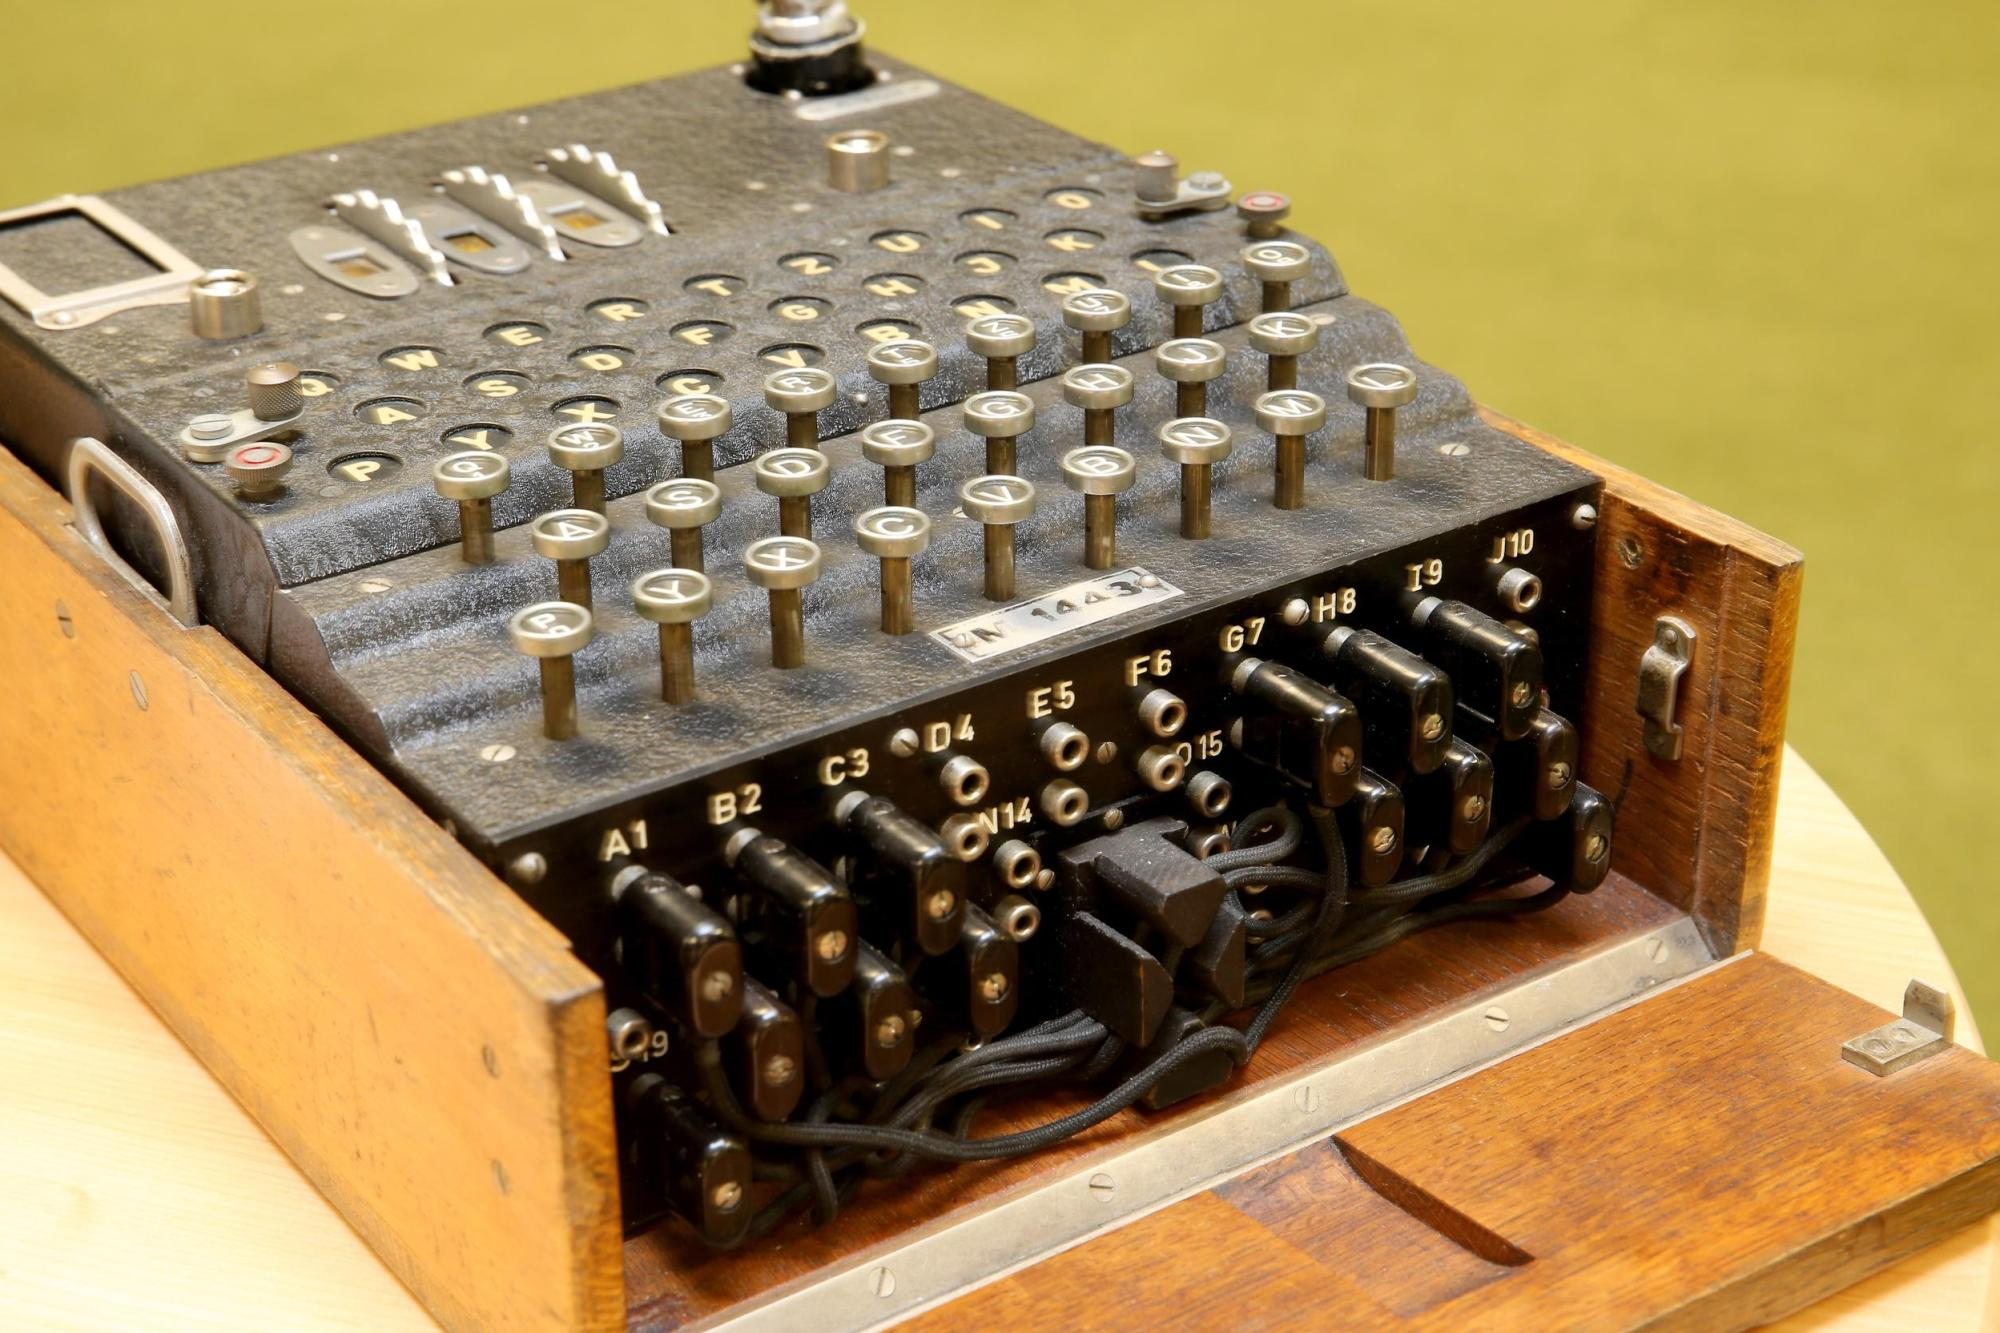
\includegraphics[width=0.7\textwidth]{bilder/enigma_stecker.jpg}
	\caption{Enigma-Maschine mit Steckerbrett, Tastenfeld und Walzen. Quelle: \cite{welt:enigma}}
	\label{fig:enigma_overview}
\end{figure}

Wird eine Taste gedrückt, fließt ein elektrischer Strom durch die Maschine und endet bei einer Lampe, die den verschlüsselten Buchstaben anzeigt. Die Walzen rotieren, sodass selbst identische Klartextzeichen unterschiedliche Chiffren erzeugen. Um eine Nachricht zu entschlüsseln, muss die Enigma in dieselbe Ausgangskonfiguration versetzt werden, mit der die Verschlüsselung erfolgte.


\newpage
\subsubsection{Komponenten der Enigma} 
Die Enigma~I verfügt über einen Walzensatz von fünf verschiedenen \textbf{Walzen (engl. rotors)}, nummeriert mit römischen Ziffern I–V. Aus diesem Satz werden drei Walzen ausgewählt und in einer bestimmten Reihenfolge in die drei Walzenplätze der Maschine eingesetzt. Diese Auswahl und Reihenfolge bezeichnet man als \textbf{Walzenlage}. Die Walzen sind jeweils auf der einen Seite mit flachen Kontakten und auf der anderen mit federbelasteten Stiften versehen. Durch die interne Verdrahtung der Walzen wird jeder Buchstabe auf genau einen anderen abgebildet. Je nach Drehung der Walze ändert sich die Abbildung.

Jede Walze besteht aus einem festen Verdrahtungskern sowie einem drehbaren äußeren Ring, auf dem Zahlen angebracht sind. Dieser äußere Ring trägt eine \textbf{Kerbe (engl. notch)}, die bestimmt, wann die nachfolgende Walze beim Tastendruck mitrotiert.

\textbf{Walzenstellung} (engl. rotor position) bezeichnet die jeweils aktuelle Position der Walze im Betrieb – also welcher Buchstabe gerade oben im Sichtfenster angezeigt wird. Nach jedem Tastendruck wird die rechte (schnelle) Walze um einen Buchstaben weitergedreht. Die anderen Walzen drehen sich nur, wenn die vorherige Walze ihre Einkerbung erreicht hat.  


\textbf{Ringstellung} (engl. ring position) beschreibt hingegen die Position der inneren Verdrahtung relativ zum äußeren Ring mit Buchstaben. Sie legt damit fest, an welcher Buchstabenposition sich die Schaltkerbe befindet und wie der elektrische Signalweg durch die Walze verläuft. Die Ringstellung wird vor dem Einsatz mechanisch über eine Schraube verstellt und bleibt während des Betriebs konstant. Sie beeinflusst sowohl den Verschlüsselungsweg als auch das Schaltverhalten der Maschine.

Die Unterscheidung zwischen Walzenstellung und Ringstellung ist entscheidend: Während die Walzenstellung angibt, wo sich die Walze gerade befindet, legt die Ringstellung fest, wie ihre interne Verdrahtung zum sichtbaren Alphabet ausgerichtet ist.

Die Kombination aus \textbf{Walzenlage}, \textbf{Walzenstellung} und \textbf{Ringstellung} wird als \textbf{Walzenkonfiguration} bezeichnet.

\begin{figure}[H]
	\centering
	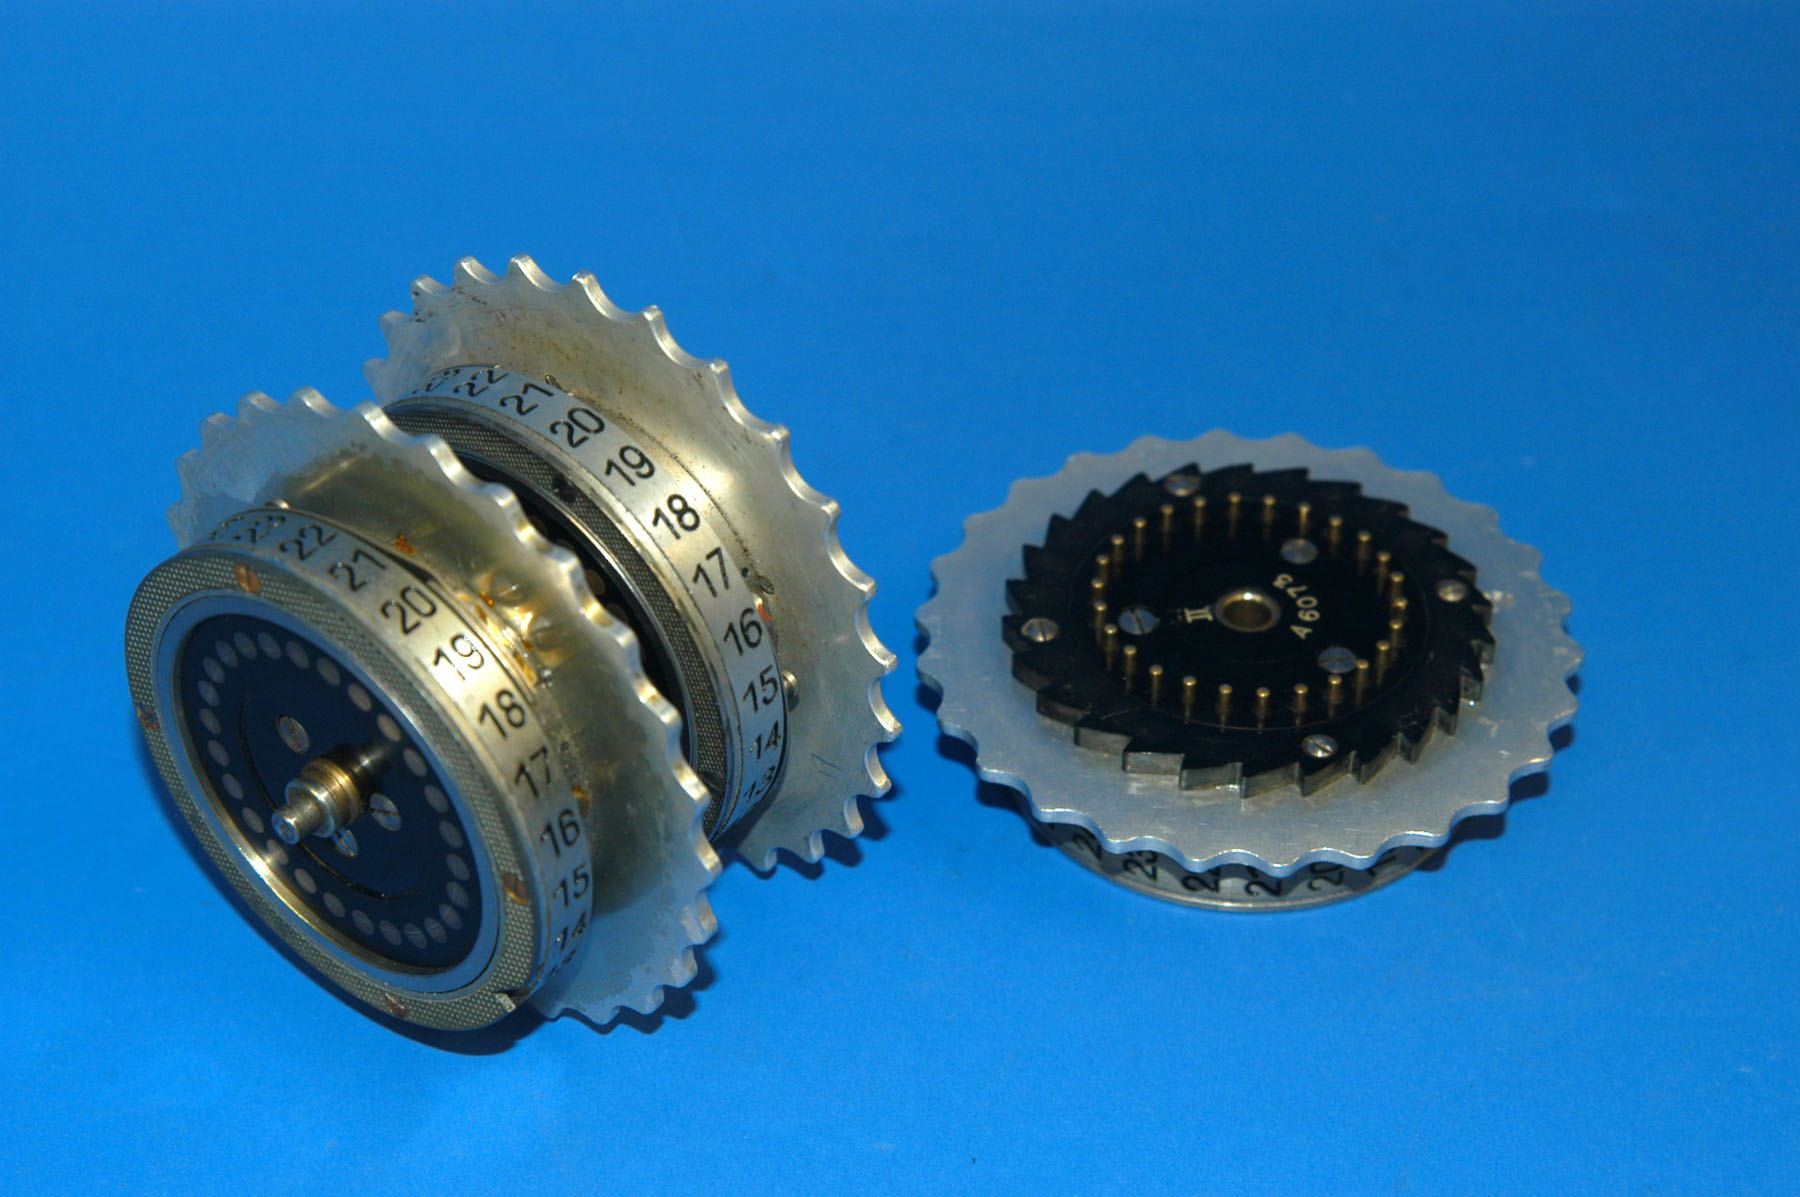
\includegraphics[width=1\textwidth]{bilder/Enigma_rotor.jpg}
	\caption{Enigma-Walze mit Einkerbung und Ring. Quelle: \cite{wiki:enigma_walzen}}
	\label{fig:Explosionsansicht}
\end{figure}

Abbildung~\ref{fig:Explosionsansicht} zeigt drei Walzen. Auf der linken Walze ist die Schaltkerbe gut zu erkennen. Ebenfalls zu sehen sind die flachen Kontakte auf der einen und die Stifte auf der anderen Seite der Walzen. Die \textbf{Walzenstellung} selbst wird hingegen erst in der Enigma-Maschine durch das Sichtfenster sichtbar.

Die \textbf{Eintrittswalze (ETW)} verbindet das Steckerbrett mit der ersten rotierenden Walze. Sie bildet das Alphabet 1:1 ab, rotiert selbst nicht und besitzt daher keine kryptografische Wirkung, wohl aber eine fest verdrahtete Zuordnung der Kontakte.

Am Ende des Stromkreises reflektiert die \textbf{Umkehrwalze (UKW, engl. reflector)} das elektrische Signal zurück durch die Walzenkette. Sie ist fest eingebaut und sorgt durch ihre Verdrahtung dafür, dass kein Buchstabe auf sich selbst abgebildet werden kann – eine charakteristische Eigenschaft der Enigma-Verschlüsselung.

Das \textbf{Steckerbrett (engl. plugboard)} besitzt 26 Buchstabenanschlüsse. Mit bis zu 13 Kabelverbindungen können Buchstabenpaare vertauscht werden (z.\,B. A $\leftrightarrow$ G). Diese Substitution findet sowohl auf dem Hin- als auch auf dem Rückweg des Signals statt und erhöht die kombinatorische Komplexität der Maschine.


\newpage
\subsubsection{Verschlüsselungsablauf}

Der Ablauf der Verschlüsselung eines einzelnen Zeichens gestaltet sich wie folgt:

\begin{figure}[H]
	\centering
	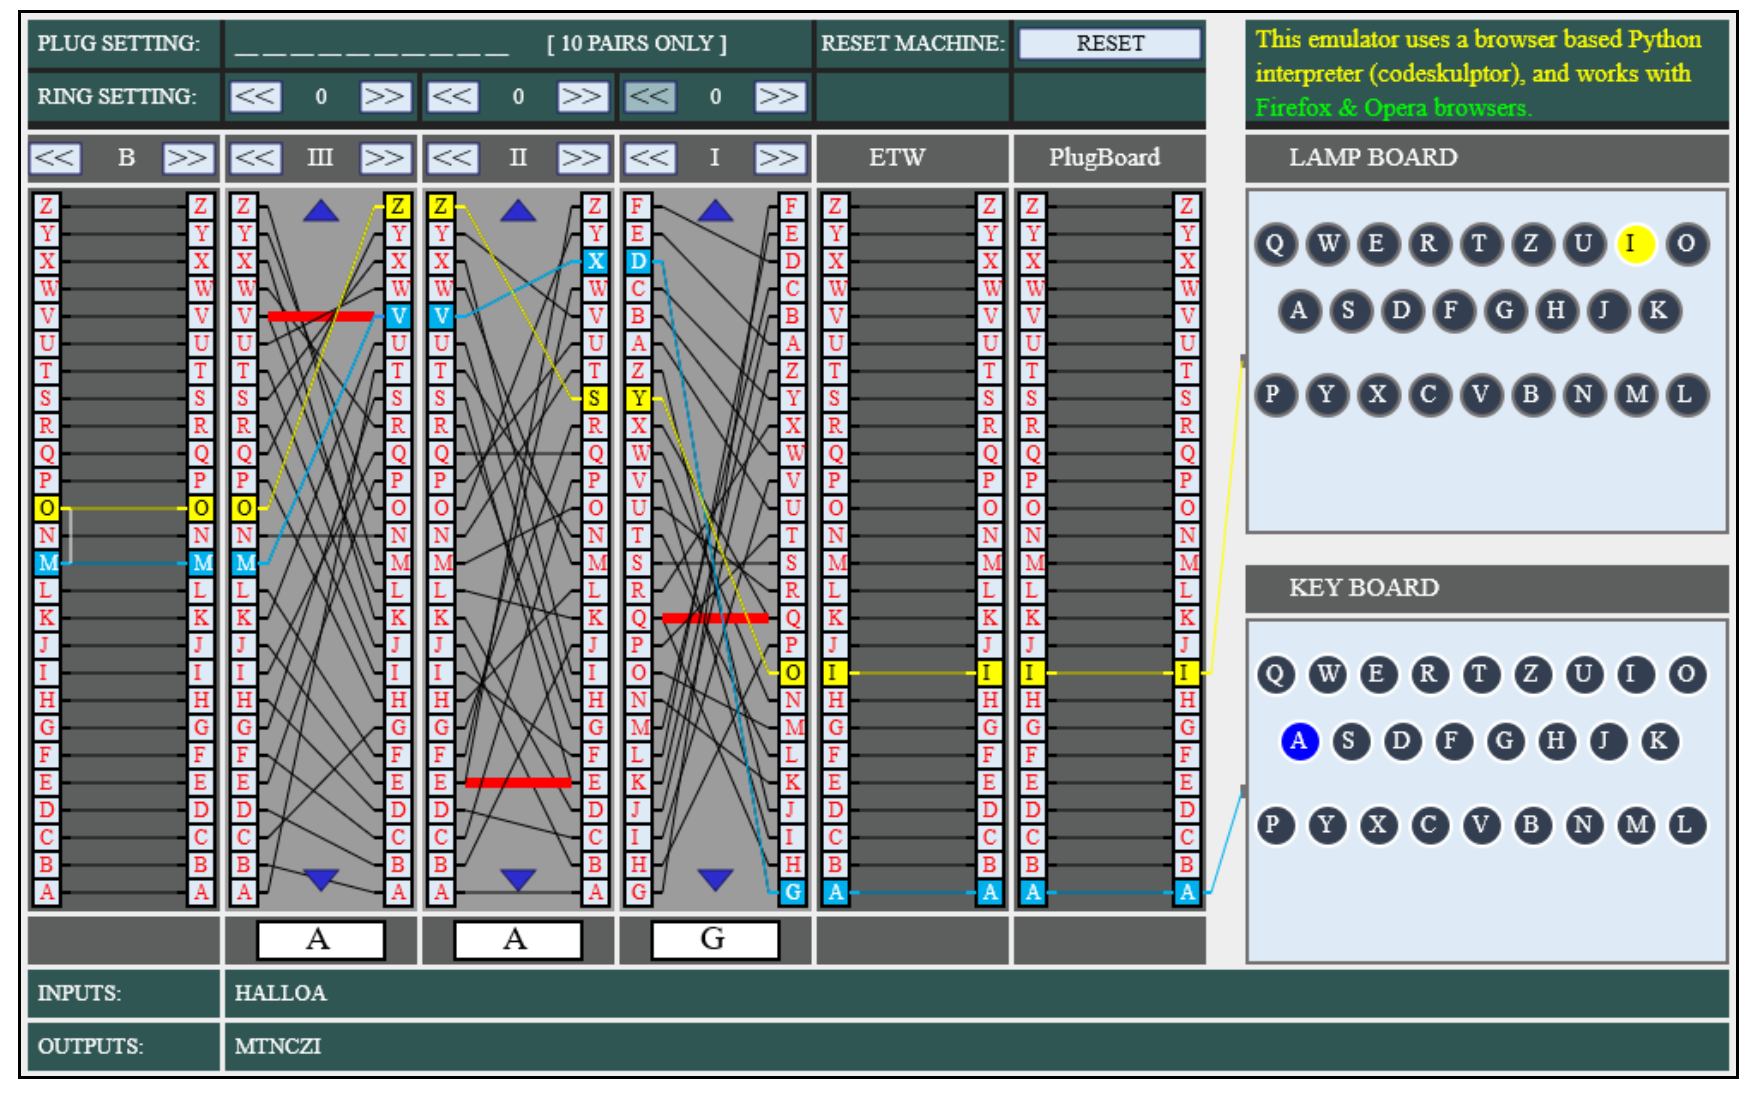
\includegraphics[width=1\textwidth]{bilder/simulator.png}
	\caption{Ablauf der Verschlüsselung. Quelle: \cite{piotte:enigma}}
	\label{fig:verschluesselungsablauf}
\end{figure}



In Abbildung~\ref{fig:verschluesselungsablauf} ist der genaue Ablauf der Verschlüsselung visualisiert. Die blaue Linie stellt den Signalweg vom Eingabebuchstaben durch die Walzen zur Umkehrwalze dar, während die gelbe Linie den Rückweg von der UKW zurück zum Lampenfeld zeigt. Die roten Markierungen auf den Walzen symbolisieren die Einkerbungen, die den Signalfluss beeinflussen. Im Folgenden wird der Verschlüsselungsprozess Schritt für Schritt erläutert:


\begin{enumerate}
	\item Konfiguration des Steckerbretts.
	\item Einstellung der Ringstellungen und Walzenlage.
	\item Einsetzen der Walzen in die Maschine.
	\item Drücken einer Taste am Tastenfeld.
	\item Die erste Walze rotiert, ggf. folgen weitere Walzen.
	\item Das elektrische Signal durchläuft nacheinander:
	\begin{itemize}
		\item das Steckerbrett,
		\item die Eintrittswalze,
		\item die drei rotierenden Walzen (Hinweg),
		\item die Umkehrwalze,
		\item die drei Walzen (Rückweg),
		\item die Eintrittswalze (Rückweg),
		\item das Steckerbrett (Rückweg).
	\end{itemize}
	\item Die entsprechende Lampe leuchtet auf und zeigt den verschlüsselten Buchstaben an.
\end{enumerate}


\subsubsection{Varianten der Enigma}

Die \textbf{Enigma M3} stellt eine Weiterentwicklung der Enigma~I dar und basiert auf demselben kryptographischen Prinzip. Diese verwendet drei Walzen, die aus einem Walzensatz von acht statt fünf Walzen ausgewählt werden. Durch die erweiterte Auswahl und variable Reihenfolge der Walzen wird die Anzahl möglicher Schlüsselkonfigurationen signifikant erhöht.


Die \textbf{Enigma M4} ersetzt die M3-Umkehrwalze durch eine zusätzliche, vierte Walze und eine schmalere Umkehrwalze, die ausschließlich an dieser Position verwendet werden können. Die ersten drei Walzen entsprechen physisch und funktional denen der M3. Die vierte Walze ist schmaler, besitzt keine Ringstellung, rotiert nicht mit und ist nicht mit den ersten drei Walzenplätzen kompatibel.

Für die vierte Position stehen zwei Walzen (\lstinline|Beta|, \lstinline|Gamma|) und zwei schmale Umkehrwalzen (\lstinline|UKW-b|, \lstinline|UKW-c|) zur Verfügung, die beliebig kombiniert werden können. Zur Abwärtskompatibilität mit der M3 wird die Walze \lstinline|Beta| in Stellung 'A' fixiert und mit der \lstinline|UKW-b| kombiniert. Analog gilt dies für \lstinline|Gamma| und \lstinline|UKW-c|.



\paragraph{Beispielrechnung zur Walzenwahl:}

Die Anzahl der möglichen Anordnungen von Walzen ergibt sich aus zwei Schritten:

\begin{enumerate}
	\item \textbf{Auswahl} von $k$ Walzen aus $n$ verfügbaren Walzen (ohne Beachtung der Reihenfolge):  
	\[
	\binom{n}{k}
	\]
	
	\item \textbf{Anordnung} der ausgewählten $k$ Walzen (alle Permutationen):  
	\[
	k!
	\]
\end{enumerate}

Die Gesamtanzahl möglicher Walzenlagen ergibt sich somit zu:
\[
\text{Walzenlagen} = \binom{n}{k} \cdot k!
\]

\newpage
Beispiele:

\begin{itemize}
	\item Drei aus drei Walzen: \(\binom{3}{3} \cdot 3! = 1 \cdot 6 = 6\)
	\item Drei aus fünf Walzen: \(\binom{5}{3} \cdot 3! = 10 \cdot 6 = 60\)
	\item Drei aus acht Walzen: \(\binom{8}{3} \cdot 3! = 56 \cdot 6 = 336\)
\end{itemize}

Wenn zusätzlich bei der Enigma~M4 eine von zwei extra dünnen Walzen sowie eine von zwei möglichen Umkehrwalzen (UKW) gewählt werden kann, erweitert sich die Gesamtanzahl möglicher Walzenkonfigurationen zu:

\[
\text{Permutationen Enigma~M4} = \underbrace{\binom{8}{3} \cdot 3!}_{\text{Walzenlagen}} \cdot \underbrace{2}_{\text{dünne Walze}} \cdot \underbrace{2}_{\text{UKW}} = 336 \cdot 2 \cdot 2 = 1344
\]




\subsection{Das Zyklometer}

Das \textbf{Zyklometer} ist eine von Marian Rejewski entwickelte elektromechanische Vorrichtung zur Entzifferung des Tagesschlüssels der Enigma. Rejewski erkannte einen sicherheitstechnischen Fehler im deutschen Verschlüsselungsverfahren, der als Grundlage für dieses Verfahren diente.

\subsubsection{Der Fehler im deutschen Verschlüsselungsverfahren}

Für den täglichen Betrieb der Enigma verwendete die deutsche Wehrmacht Codebücher, welche die Walzenlage, Walzenstellung, Ringstellung und die Steckerbrettverbindungen für jeden Tag enthielten. Diese Gesamtheit der Einstellungen wird als Tagesschlüssel bezeichnet. 

%\begin{itemize}
%	\item Der Absender stellt seine Enigma-Maschine gemäß des Tagesschlüssels ein und übermittelt eine beliebige Walzenstellung für der Nachricht selbst (z.\,B.\ \lstinline|"ABC"|) zweimal hintereinander (hier \lstinline|"ABCABC"|). Dieses übermitteln der Walzenstellung wird auch \textbf{Spruchschlüssel} genannt. Dieser ist nur für die Länge der Nachricht gültig.
%	\item Anschließend wird die Walzenstellung entsprechend dem Spruchschlüssel vom Absender eingestellt.
%	\item Der Empfänger stellt seine Enigma-Maschine gemäß des Tagesschlüssels ein und entschlüsselte die ersten sechs Buchstaben, welche dem Spruchschlüssel entsprachen.
%	\item Anschließend stellt der Absender die Walzenstellung entsprechend dem Spruchschlüssel ein und dechiffrierte die Nachricht.
%\end{itemize}


Zur Sicherung einzelner Nachrichten wählte der Absender eine eigene Walzenstellung, welche mit drei Buchstaben beschrieben (z.\,B.\ \lstinline|"ABC"|) und als \textbf{Spruchschlüssel} bezeichnet wurde. Dieser Spruchschlüssel wurde verdoppelt (z.\,B.\ \lstinline|"ABCABC"|), mit dem Tagesschlüssel verschlüsselt, übertragen. Der Empfänger konnte durch Entschlüsselung der ersten sechs Zeichen den Spruchschlüssel rekonstruieren, die Maschine entsprechend einstellen und die Nachricht dechiffrieren.

Das doppelte Übertragen des Spruchschlüssels erzeugte allerdings eine feste Zuordnung zwischen den Buchstabenpositionen 1 und 4, 2 und 5 sowie 3 und 6 einer jeden Nachricht eines Tages. Dieser systematische Aufbau offenbarte eine wiederkehrende Struktur, die – unter kryptoanalytischem Blickwinkel – gezielt ausgewertet und als Angriffsvektor verwendet werden konnte.



\subsubsection{Zyklenbildung aus Spruchschlüsseln}
Diesen Umstand erkannten bereits in den 1930er-Jahren die polnischen Kryptologen als zentrale Schwachstelle der Enigma. Ihre Analyse führte zur Entwicklung einer Methode, mit der sich aus verschlüsselten Spruchschlüsseln charakteristische Muster ableiten ließen. 

Dabei wurden aus der verdoppelten Übertragung (z.\,B.\ \textbf{"ABCABC"}\newline $\rightarrow$ \textbf{"BJEGSM"}) charakteristische Buchstabenpaare an den Positionen 1:4, 2:5 und 3:6 extrahiert – im Beispiel also \textbf{B:G}, \textbf{J:S} und \textbf{E:M}.

Diese Zuordnungen lassen sich in sogenannte \textbf{Zyklen} überführen. Betrachtet man beispielsweise das Buchstabenpaar \textbf{B:G} (aus Position 1:4), so wird analysiert, welchem Buchstaben \textbf{G} seinerseits zugeordnet ist – z.\,B.\ in einem weiteren Paar \textbf{G:F}. Daraus ergibt sich die Sequenz \textbf{B}~$\rightarrow$~\textbf{G}~$\rightarrow$~\textbf{F}. Findet sich nun noch ein drittes Paar \textbf{F:B}, so schließt sich der Zyklus: \textbf{B}~$\rightarrow$~\textbf{G}~$\rightarrow$~\textbf{F}~$\rightarrow$~\textbf{B}. Es entsteht ein geschlossener Zyklus der Länge drei.

Wichtig dabei ist, dass jeder Buchstabe im Alphabet genau einmal in einer Zuordnung vorkommt. Deshalb ist eine ausreichende Anzahl an abgefangenen Spruchschlüsseln erforderlich. Es handelt sich um eine Permutation, bei der keine Buchstaben doppelt verwendet werden dürfen – weder als Ausgangs- noch als Zielbuchstabe innerhalb desselben Zyklenbaums.


Dieser Vorgang wird getrennt für jede der drei Positionspaarungen (1:4, 2:5, 3:6) durchgeführt. Für jede dieser Zuordnungsgruppen entsteht dabei eine eigene Zyklenstruktur. Man erhält somit pro Nachricht drei charakteristische Zyklenmengen, die getrennt analysiert werden.

Das Verfahren wird auf alle Buchstabenpaare angewendet, bis das gesamte Alphabet in disjunkte Zyklen eingeteilt ist. Die Gesamtheit dieser Zyklen bezeichnet man als \textbf{Charakteristik}.

Durch die doppelte Übertragung des Spruchschlüssels entstehen jeweils zwei zueinander inverse Permutationen mit identischer Zyklenstruktur. Daher tritt jede Zyklencharakteristik im Zyklometer in doppelter Ausführung auf.

\newpage
\subsubsection{Technische Umsetzung des Zyklometers}

Um diesen Prozess zu automatisieren, entwickelte Rejewski schließlich das \textbf{Zyklometer} – ein elektromechanisches Gerät, das im Kern aus zwei hintereinandergeschalteten Enigma-Walzen besteht, wobei die zweite Walze um drei Positionen weitergedreht ist. So konnten systematisch die möglichen Zyklen für alle Walzenstellungen berechnet und dokumentiert werden.


\begin{figure}[H]
	\centering
	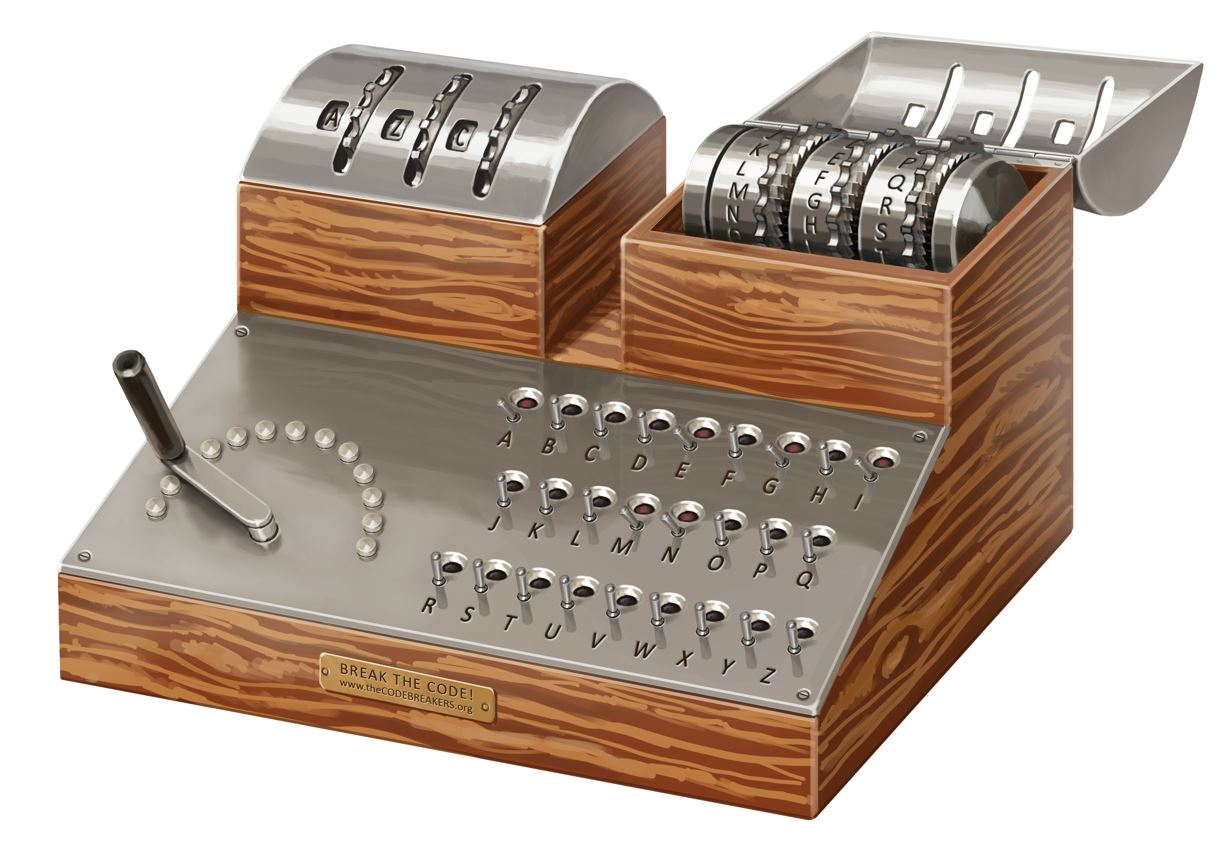
\includegraphics[width=0.7\textwidth]{bilder/Zyklometer.jpg}
	\caption{Zyklometer Quelle: \cite{wiki:zyklometer}}
	\label{fig:Zyklometer}
\end{figure}

In Abbildung~\ref{fig:Zyklometer} ist ein Zyklometer zu sehen. Jeder Buchstabe ist mit einem Schalter und einer Lampe ausgestattet. Wenn der Schalter eines Buchstabens betätigt wird, leuchten alle Buchstaben auf, die zusammen mit dem gewählten Buchstaben einen Zyklus bilden. Die Anzahl der leuchtenden Buchstaben entspricht dabei der Zykluslänge.






\subsubsection{Katalog der Charakteristiken}

Im Katalog der Charakteristiken werden alle Zyklen der Enigma~I-Permutationen bei neutraler Ringstellung und Umkehrwalze UKW-B dokumentiert. Ist die tatsächliche Ringstellung bekannt, lässt sich ihr Einfluss durch Subtraktion der Ringstellung von der Walzenstellung (modulo~26) kompensieren. So bleibt der Abgleich mit dem Katalog gültig.



Der Katalog umfasst alle möglichen Permutationen. Insgesamt enthält der er \(63\,420\) eindeutig unterschiedliche Zyklenlängen-Charakteristiken.



\newpage
Die Gesamtzahl der möglichen Enigma~I-Permutationen ergibt sich aus der Anzahl der Walzenlagen, Walzenstellungen und Ringstellungen:

\[
\text{Walzenlagen} = \binom{5}{3} \cdot 3! = 10 \cdot 6 = 60
\]
\[
\text{Walzenstellungen} = 26^3 = 17\,576
\]
\[
\text{Ringstellungen} = 26^3 = 17\,576
\]

\[
\text{Die Gesamtanzahl der Konfigurationen} = 60 \cdot 17\,576 \cdot 17\,576 \approx 18{,}5 \text{ Milliarden}
\]

Da die Ringstellung in der Analyse als bekannt vorausgesetzt wird, reduziert sich die Anzahl auf:
\[
60 \cdot 17\,576 = 1\,054\,560
\]

\paragraph{Abgleich Walzenlage und Walzenstellung:}

Diesen über einer Million Konfigurationen stehen \(63\,420\) verschiedene mögliche \textbf{Zyklenlängen\hyp{}Charakteristiken} gegenüber. Damit reduziert sich die Anzahl potenzieller Walzenkonfigurationen pro Charakteristik auf durchschnittlich etwa \(\frac{1\,054\,560}{63\,420} \approx 16{,}6\) Kandidaten. Durch den Vergleich der Zyklenlängen der verschlüsselten Nachricht mit dem Katalog lässt sich die Menge der möglichen Konfigurationen somit deutlich eingrenzen.


\paragraph{Analyse des Steckerbretts:}

Das Steckerbrett verändert nicht die Längen der Zyklen, sondern lediglich deren innere Struktur. Daher können aus den Zyklenlängen die Walzenlage und -stellung unabhängig von den Steckerbrettverbindungen ermittelt werden.

Letzere werden anhand der Zyklenstrukturen analysiert. Dabei muss jedoch zunächst die korrekte Walzenlage und -stellung bekannt und eingestellt sein. Anschließend werden die Zyklenstrukturen, wie sie ohne Steckerbrettverbindungen im Katalog vorliegen, mit denen aus den abgefangenen Nachrichten verglichen.

\paragraph{Bestimmung der Ringstellung:}

Eine direkte Bestimmung der Ringstellung mit dem Zyklometer ist nicht möglich. Stattdessen wurde die Ringstellung durch systematisches Ausprobieren aller $26^3$ Kombinationen mithilfe der von Rejewski entwickelten \textbf{Grill-Methode} ermittelt. Diese Methode nutzte die Annahme, dass viele Nachrichten mit dem bekannten Präfix \textbf{"ANX"} (Leerzeichen als  \textbf{"X"} geschrieben) begannen, was die Suche erheblich erleichterte \autocite{rejewski1981enigma}.



\subsection{Bedeutung des Zyklometers}

Das Zyklometer stellte eine zentrale methodische Innovation im Kampf gegen die Verschlüsselung durch die Enigma dar. Entwickelt und eingesetzt von den polnischen Kryptographen, insbesondere Marian Rejewski, ermöglichte es eine systematische Analyse der durch die Enigma erzeugten Permutationen. Die Erstellung eines Katalogs von Zyklencharakteristiken reduzierte die enorme Komplexität der möglichen Walzenkonfigurationen und erlaubte erstmals die gezielte Bestimmung von Schlüsseln.

Diese Vorarbeiten bildeten die Grundlage für spätere Erfolge der britischen Kryptanalytiker um Alan Turing in Bletchley Park. Die Konstruktion der elektromechanischen Entschlüsselungsmaschine \textbf{Turing-Welchman-Bombe} baute direkt auf den Konzepten des Zyklometers auf und überführte sie in eine automatisierte Form. Somit markierte das Zyklometer einen entscheidenden Meilenstein auf dem Weg zur erfolgreichen Entzifferung der Enigma.





\section{Technische Vorarbeiten und Codebasis}
\label{sec:analyse_c_implementation}

Die technische Grundlage der vorliegenden Arbeit bildet eine in mehreren Phasen weiterentwickelte C-Implementierung der Enigma-Maschine. Diese wurde im Laufe verschiedener studentischer Projekte schrittweise erweitert und verbessert.

Den Ausgangspunkt bildete eine erste Version der Simulation, die von Arif Hasanic entwickelt wurde. Diese umfasste eine funktionale Nachbildung sowohl der Enigma-Maschine als auch des Zyklometers\autocite{hasanic2024enigma}.

Aufbauend auf dieser Codebasis erstellte Emanuel Schäffer im Rahmen seiner eigenen Arbeit eine erweiterte Version. Diese beinhaltete neben Verbesserungen in Typsicherheit, Speicherverwaltung und Codequalität auch die Simulation der Turing-Welchman-Bombe\autocite{schaffer2025enigma}.

Für die vorliegende Arbeit wurde schließlich ein Fork dieser erweiterten Implementierung angelegt, der von Emanuel Schäffer und mir gemeinsam weiterentwickelt worden ist\autocite{schaffer2025enigmaserver}. Diese dritte Entwicklungsstufe bildet die Grundlage für die hier vorgestellten Analyse- und Erweiterungsschritte.



\newpage
\section{Konzeption der Anwendung}

Dieses Kapitel beschreibt die Architektur und den Betrieb der Anwendung. Zunächst wird der logische Aufbau erläutert, also wie die einzelnen Komponenten zusammenspielen. Anschließend folgt eine Beschreibung der konkreten Umsetzung auf Serverebene.

\subsection{Architekturüberblick}

Die Anwendung ist modular aufgebaut und besteht aus vier Hauptkomponenten:

\begin{itemize}
	\item \textbf{Frontend:} Browserbasierte Single-Page Application (SPA).
	\item \textbf{Backend:} Java-Anwendung mit Spring Boot.
	\item \textbf{Native Bibliothek:} In C geschriebene Shared Library für kryptografische Berechnungen.
	\item \textbf{Datenbank:} Relationale PostgreSQL-Datenbank.
\end{itemize}

Alle Komponenten kommunizieren über klar definierte Schnittstellen. Das Frontend nutzt eine HTTP-Schnittstelle zur Interaktion mit dem Backend. Das Backend greift über das Java Foreign Function \& Memory API (FFM API) direkt auf die native Bibliothek zu. Die Datenbank wird ausschließlich über JDBC angesprochen. Innerhalb des Backends sind diese Funktionalitäten modular getrennt, was die Wartbarkeit verbessert.


\begin{figure}[H]
	\centering
	\begin{tikzpicture}[
		node distance=1.5cm and 3cm,
		box/.style={draw, rounded corners, minimum width=4cm, minimum height=1.2cm, align=center},
		arrow/.style={-Latex, thick, font=\small}
		]
		% Oben
		\node[box] (frontend) {nginx Frontend};
		% Direkt darunter
		\node[box, below=of frontend] (backend) {Java Spring Boot Backend};
		% Darunter nebeneinander
		\node[box, below=3cm of backend, xshift=-2.5cm] (db) {PostgreSQL-Datenbank};
		\node[box, below=3cm of backend, xshift=2.5cm] (native) {Native Bibliothek};
		
		% Vertikale Pfeile mit Text rechts
		\draw[<->, thick] (frontend) -- node[right] {HTTP API (REST)} (backend);		
		\draw[<->, thick] (backend) -- node[left] {JDBC / Hibernate } (db);
		\draw[<->, thick] (backend) -- node[right] { FFM API} (native);
	\end{tikzpicture}
	\caption{Architektur der Anwendung mit Schnittstellen}
	\label{fig:architektur-schnittstellen}
\end{figure}


Die Anwendung unterstützt drei zentrale Funktionen: Verschlüsselung, Zyklenerzeugung und Katalogabfrage. 
Die ersten beiden werden über die native Bibliothek im Backend berechnet, während die Katalogabfrage über die PostgreSQL-Datenbank erfolgt.

\subsection{Betrieb und Hostingstrategie}

Die Anwendung wird vollständig auf einem dedizierten Ubuntu-Server (ein Linux-basiertes Betriebssystem) der Hochschule Ravensburg-Weingarten betrieben. Die Bereitstellung erfolgt mit Hilfe etablierter Open-Source-Komponenten:

\begin{itemize}
	\item \textbf{Frontend:} \lstinline|nginx| übernimmt das Routing eingehender HTTP-Anfragen (Stan\-dard-Port 80 für Webverkehr) und dient sowohl als Reverse-Proxy als auch als Webserver für die statischen Frontend-Dateien. Konfiguration unter \lstinline|/etc/nginx/sites-available/enigma|, Inhalte unter \lstinline|/var/www/enigma|.	
	
	\item \textbf{Backend:} Die Spring Boot-Anwendung (Version~3.4.5, kompiliert mit Java~23) liegt als ausführbare JAR unter \lstinline|/opt/enigma/enigma_api.jar| vor. Sie wird als systemd-Dienst auf dem lokalen Port 8081 betrieben (\lstinline|/etc/systemd/system/enigma.service|) und kommuniziert mit der C-Bibliothek \lstinline|/opt/enigma/enigma_c/libenigma.so| sowie der PostgreSQL-Datenbank. \newline HTTP-Kompression und Caching sind aktiviert.
	
	\item \textbf{Datenbank:} PostgreSQL~17.5 läuft lokal auf dem Server an Port 5432 und ist ausschließlich für das Backend zugänglich. Genutzt wird die Datenbank \lstinline|catalogue|.
	
	\item \textbf{Netzwerkanbindung:} Der Server ist über einen hochschulinternen Reverse-Proxy erreichbar. Zugriffsbeschränkungen über IP-Filter, VPN oder Authentifizierung sind derzeit nicht implementiert.
\end{itemize}


\newpage
\section{Anpassungen des C-Quellcodes}
\label{sec:c_modifications}

Aufbauend auf der in Kapitel \ref{sec:analyse_c_implementation} beschriebenen Codebasis wurden im Rahmen dieser Arbeit verschiedene Erweiterungen und strukturelle Verbesserungen am bestehenden C-Quellcode vorgenommen. Ziel dieser Maßnahmen war es, die bestehende Funktionalität robuster und flexibler zu gestalten sowie eine problemlose Integration in eine moderne Systemarchitektur zu ermöglichen.

Die vorgenommenen Änderungen lassen sich im Wesentlichen in drei Bereiche unterteilen:
\begin{itemize}
	\item strukturelle und funktionale Optimierungen,
	\item Erweiterungen zur Generierung von Datenbankinhalten,
	\item Modularisierung für die Anbindung an einen HTTP-Controller.
\end{itemize}



\subsection{Strukturelle Optimierungen und Refactoring}
\label{subsec:c_structural}

Die internen Datenstrukturen wurden überarbeitet: Ursprünglich wurden Permutationen der Walzenlagen als \lstinline|char|-Arrays mit 26 Elementen gespeichert, was wiederholte Umrechnungen zwischen Zeichen und Indizes erforderte und potenzielle Fehlerquellen eröffnete. Die Umstellung auf ein integerbasiertes \lstinline|RotorPermutations|-Struct erlaubt nun direkte Indexzugriffe und vereinfacht die Zyklusberechnung.

Darüber hinaus wurde die Zyklusberechnung selbst überarbeitet. Die ursprüngliche Funktion \lstinline|find_cycle_lens| wurde durch \lstinline|calculate_cycle_len| ersetzt, welche speziell auf integerbasierte Permutationen ausgelegt ist und Fehlerzustände wie ungültige Indizes (z.\,B. \lstinline|-1|) zuverlässiger erkennt und behandelt. 

Auch die Speicherverwaltung wurde robuster gestaltet: Durch die Festlegung einer maximalen Anzahl von Tagesschlüsseln können Speicherüberläufe verhindert werden. 

Diese Anpassungen wurden im Rahmen gemeinsamer Weiterentwicklung mit Emanuel Schäffer vorgenommen. 


\newpage
\subsection{Erweiterungen für die Datenbankgenerierung}
\label{subsec:c_db_export}

Zur Erstellung eines Katalogs der charakteristischen Zyklen aller möglichen Walzenkonfigurationen wurde das Programm in ein eigenständiges Kommandozeilenwerkzeug überführt. Dieses nimmt eine Zieldatei als Argument entgegen und schreibt die Ergebnisse direkt in eine Textdatei. Der anschließende Import dieser Datei in eine relationale PostgreSQL-Datenbank wird im Kapitel \ref{sec:db_erstellung} erläutert.


Ziel dieser Erweiterung ist es, für alle Kombinationen aus Walzenlage und Walzenstellung, die charakteristischen Zyklen zu ermitteln. Das Kernprinzip des Algorithmus umfasst folgende Schritte:

\begin{enumerate}
	\item Für jede Walzenlage werden alle Permutationen generiert \newline(\lstinline|generate_permutations|), also \(\binom{5}{3} \cdot 3! = 60\).
	\item Für jede Walzenlage werden alle $26^3 = 17\,576$ Walzenstellungen (von \lstinline|AAA| bis \lstinline|ZZZ|) durchlaufen.
	\item Für jede dieser Konfigurationen werden 26 Spruchschlüssel (\lstinline|"AAAAAA"| bis \newline\lstinline|"ZZZZZZ"|) verschlüsselt, wobei Ringstellung und Steckerverbindungen konstant bleiben.
	\item Aus diesen verschlüsselten Schlüsseln werden die Zyklen bestimmt \newline(\lstinline|calculate_cycle_lengths|).
	\item Die Ergebnisse werden in einer Textdatei persistiert (\lstinline|print_whole_cycle|).
\end{enumerate}

Die Ausgabe enthält $60 \cdot 17\,576 = 1\,054\,560$ Zeilen, wobei jede Zeile die folgenden Informationen umfasst:

\begin{itemize}
	\item Drei Arrays mit Zyklenlängen,
	\item Die Walzenstellung im Klartext (\lstinline|AAA| bis \lstinline|ZZZ|),
	\item Die Walzenlage als Integer-Array.
\end{itemize}

\lstinline|{12,12,1,1};{12,12,1,1};{7,7,3,3,2,2,1,1};ABC;{1,2,3}|

Die obige Zeile beschreibt eine Enigma-Konfiguration mit der Walzenlage \lstinline|{1,2,3}| und der Walzenstellung \lstinline|"ABC"| sowie den jeweils ermittelten Zyklenlängen. Die Wiederholung gleicher Zyklenlängen innerhalb einer Permutation ist dabei zulässig.

\newpage

\subsection{Modularisierung für die Anbindung an einen HTTP-Controller}  
\label{subsec:c_api_prep}

Im Rahmen der Integration der Enigma-Funktionalität in eine moderne Web\-architektur wurde der C-Code so angepasst, dass zentrale Funktionen wie \lstinline|enigma_encrypt|, \lstinline|calculate_cycle_lengths| und \lstinline|rotor_mapping| als klar modularisierte, aufrufbare Einheiten vorliegen. Diese Modularisierung ermöglicht es, die Enigma-Logik bequem und zuverlässig von einem HTTP-Controller aus aufzurufen.

Um die Wartbarkeit und Parallelisierbarkeit zu erhöhen, wurde bewusst auf den Einsatz von globalen Zuständen verzichtet, also Variablen, die außerhalb von Funktionen gemeinsam genutzt werden. Stattdessen werden alle notwendigen Daten über Funktionsparameter und lokale Variablen verwaltet, wodurch Seiteneffekte vermieden und die Integration in unterschiedliche Softwareumgebungen erleichtert wird.


Zentraler Bestandteil dieser Modularisierung ist die Einführung einer strukturierten Datenstruktur \lstinline|EnigmaConfiguration|, die alle erforderlichen Parameter der Enigma-Verschlüsselung bündelt. Diese Struktur dient als Eingabe für die C-Funktionen und bildet somit eine übersichtliche Schnittstelle zwischen der nativen C-Implementierung und der höheren Anwendungsschicht, beispielsweise einem HTTP-Controller:

\begin{lstlisting}[language=C, caption={Struct \lstinline|EnigmaConfiguration| in C}, label={lst:enigma-c}]
typedef struct {
	char plugboard[26];
	char *message;
	uint8_t *rotor_positions;
	uint8_t *ring_settings;
	enum ROTOR_TYPE *rotors;
	enum ENIGMA_TYPE type;
	enum REFLECTOR_TYPE reflector;
} EnigmaConfiguration;
\end{lstlisting}

Zusätzlich wurde eine Begrenzung der Nutzeranfragen implementiert, um die Stabilität des Servers zu gewährleisten. So wird sichergestellt, dass jede Anfrage innerhalb einer kontrollierbaren Zeit beantwortet wird, was Überlastungen durch besonders rechenintensive Anfragen verhindert.

Die konkrete technische Umsetzung der Integration in höhere Softwareebenen, insbesondere die Anbindung an RESTful APIs, wird im folgenden Kapitel beschrieben.

 
\newpage


\section{Vom C-Code zur RESTful API}

Aufbauend auf den im vorherigen Kapitel beschriebenen technischen Vorarbeiten und den modularisierten Anpassungen des bestehenden C-Codes wird in diesem Abschnitt gezeigt, wie aus einer ursprünglich eigenständigen Programm-Implementierung eine native Bibliothek entwickelt wurde. Diese Bibliothek dient als Grundlage für einen RESTful Backend-Server auf Basis von Java.

Der Fokus liegt dabei auf den konzeptionellen sowie technischen Herausforderungen bei der Integration der C-Funktionalität mittels der Java Foreign Function \& Memory API (FFM API) und deren Einbindung in ein modernes Spring-Boot-Backend. So wird der Weg von einem monolithischen C-Programm hin zu einer flexiblen, webbasierten API beschrieben, die den Anforderungen moderner Webanwendungen gerecht wird.

Die in diesem Kapitel beschriebenen Entwicklungen sowie der zugehörige Code sind im begleitenden GitHub-Repository dokumentiert und verfügbar\autocite{steidle2025enigmaapi}.

\subsection{Von nativer C-Implementierung zur Foreign Function \& Memory API}
\label{subsec:ffm_evolution}

Der initiale Ansatz bestand darin, die Enigma-Funktionalität über einen in C implementierten REST-API-Server bereitzustellen. Im praktischen Einsatz zeigte sich jedoch, dass die manuelle De-/Serialisierung von JSON, die Validierung komplexer Konfigurationen sowie das Speicherzugriffsmanagement in C äußerst fehleranfällig und wartungsintensiv sind. Die experimentelle Serverimplementierung wurde daher zugunsten einer robusteren Architektur verworfen.

Alternativ wurde das Java Native Interface (JNI) evaluiert. Trotz prinzipieller Funktionalität erwies sich der damit verbundene Boilerplate-Code\footnote{Standardisierter, wiederkehrender Code, der in vielen Programmen ähnlich geschrieben werden muss, aber wenig direkte Logik enthält.}, sowie das manuelle Speicher- und Fehlerhandling und der Debugging-Aufwand als nicht zielführend. Zudem ist bei JNI häufig auch sogenannter Glue-Code\footnote{Code, der verschiedene Software-Komponenten oder Systeme miteinander verbindet und ihre Kommunikation ermöglicht.} erforderlich.


Die Wahl fiel schließlich auf die FFM API. Sie ermöglicht typsichere, speichereffiziente und performante Interoperabilität mit nativen C-Bibliotheken – ohne zusätzliche Glue-Code-Ebenen.

\newpage
\subsection{Technische Integration mit der FFM API}
\label{subsec:ffm_integration}

Die FFM API bietet mit \lstinline|MemorySegment|, \lstinline|MethodHandle| und \lstinline|FunctionDescriptor| präzise Kontrollmechanismen über Speicherlayout, Funktionssignaturen und Datenmarshalling (d.h. die Konvertierung von Java-Datenstrukturen in native Repräsentationen und umgekehrt). Zwei Funktionen wurden angebunden: \lstinline|enigma_encrypt(...)| zur Verschlüsselung sowie \newline\lstinline|manual_get_cycles_from_cyclometer(...)| zur Berechnung der Zyklenlängen.


\paragraph{Speicherabbildung der Struktur \lstinline|EnigmaConfiguration|:}
Die native C-Struktur \lstinline|EnigmaConfiguration| (siehe Abschnitt~\ref{subsec:c_api_prep}) wurde mittels \newline\lstinline|MemoryLayout.structLayout(...)| in Java modelliert. Zur Sicherstellung der korrekten Speicher-Alignment-Anforderungen wurde zwischen statischem Plugboard-Feld und Pointer-Feldern ein Padding-Segment eingefügt:

\begin{lstlisting}[language=Java, caption={FFM-Deklaration der Struktur \lstinline|EnigmaConfiguration|}, label={lst:ffm-layout}]
private static final MemoryLayout ENIGMA_LAYOUT = MemoryLayout.structLayout(
MemoryLayout.sequenceLayout(26, JAVA_BYTE).withName("plugboard"),
MemoryLayout.paddingLayout(6),
ADDRESS.withName("message"),
ADDRESS.withName("rotor_positions"),
ADDRESS.withName("ring_settings"),
ADDRESS.withName("rotors"),
JAVA_INT.withName("type"),
JAVA_INT.withName("reflector")
).withName("EnigmaConfiguration");
\end{lstlisting}

\paragraph{Aufruf der Verschlüsselungsfunktion:}
Instanzen der Struktur werden durch eine Hilfsklasse \lstinline|JavaToCFactory| erstellt. Speicherbereiche werden ASCII-kodiert allokiert, Pointer korrekt gesetzt. \newline Der Funktionsaufruf erfolgt über ein \lstinline|MethodHandle|:


\begin{lstlisting}[language=Java, caption={Aufruf der FFM-Funktion \lstinline|enigma_encrypt|}, label={lst:ffm-encrypt}]
final var enigmaSeg = EnigmaFactory.createEnigmaSegment(enigma, arena);
final var outputSeg = arena.allocate(byteSize);
final int ret = (int) ENIGMA_ENCRYPT.invoke(enigmaSeg, outputSeg);

if (ret == 0) {
	final String outputString = outputSeg.reinterpret(byteSize).getString(0);
	return Optional.of(outputString);
}
\end{lstlisting}

\newpage
\paragraph{Konvertierung von String[] nach char**:}
Zur Rotorzyklenermittlung erwartet die C-Funktion ein nullterminiertes \lstinline|char**|-Array. In Java erfolgt die Umsetzung durch ASCII-kodierte Strings, deren Adressen in einem Pointer-Array abgelegt werden. Ein NULL-Zeiger terminiert das Array:
\begin{lstlisting}[language=Java, caption=Konvertierung von String zu char**]
public static MemorySegment allocateTerminatedASCIIArrayFromStringArray(
final String[] stringArr, final Arena arena) {
	int length = stringArr.length;
	MemorySegment segment = arena.allocate(
	ValueLayout.ADDRESS.byteSize() * (length + 1),
	ValueLayout.ADDRESS.byteSize()
	);
	for (int i = 0; i < length; i++) {
		MemorySegment stringSegment = 
		allocateTerminatedASCIIFromString(stringArr[i], arena);
		segment.setAtIndex(ValueLayout.ADDRESS, i, 
		MemorySegment.ofAddress(stringSegment.address()));
	}
	segment.setAtIndex(ValueLayout.ADDRESS, length, MemorySegment.NULL);
	return segment;
}
\end{lstlisting}

\paragraph{Rückgabewert als Struktur: Cyclometer-Daten extrahieren:}
Die Funk\-tion \lstinline|manual_get_cycles_from_cyclometer| liefert eine \lstinline|ComputedCycles|-Struktur zurück. Diese wird in Java über ein entsprechendes Layout modelliert und mit \lstinline|VarHandle| feldweise gelesen:

\begin{lstlisting}[language=Java, caption=Layout des Rückgabewerts ComputedCycles]
private static final MemoryLayout CYCLOMETER_LAYOUT = MemoryLayout.structLayout(
JAVA_INT.withName("cycles_1_4_len"),
JAVA_INT.withName("cycles_2_5_len"),
JAVA_INT.withName("cycles_3_6_len"),
MemoryLayout.sequenceLayout(26, JAVA_INT).withName("cycles_1_4"),
MemoryLayout.sequenceLayout(26, JAVA_INT).withName("cycles_2_5"),
MemoryLayout.sequenceLayout(26, JAVA_INT).withName("cycles_3_6")
);
\end{lstlisting}

Die extrahierten Felder werden in ein dediziertes Java-Datenobjekt übertragen:

\begin{lstlisting}[language=Java]
return new CyclometerCycles(firstToThird, secondToFourth, thirdToSixth);
\end{lstlisting}


\paragraph{Technische Schlussfolgerungen:}

Die Java FFM API erlaubt eine technisch saubere, speichersichere und performante Anbindung nativer C-Bibliotheken. Besondere Herausforderungen bestehen in der korrekten Modellierung von Speicherstrukturen, der Zeigerarithmetik und der Datenkonversion. Durch eine strikte Modularisierung und den Einsatz von Factory-Klassen entsteht eine robuste, wartbare und portable Lösung.




\subsection{Entwicklung des Backends mit Spring Boot}

Nach der erfolgreichen Implementierung der nativen FFM-API-Schnittstelle stellte sich die Frage, wie diese als Webservice effizient bereitgestellt werden kann. Aufgrund der hohen Verbreitung, der umfangreichen Dokumentation sowie der ausgereiften Unterstützung für REST-APIs wurde Spring Boot als Framework gewählt.

\paragraph{Controller-Architektur:}

Zentrale Komponente ist der \lstinline|EnigmaController|, der die drei Hauptendpunkte \lstinline|/api/enigma|, \lstinline|/api/cyclometer| und \lstinline|/api/catalogue| bereitstellt. Diese Aufteilung gewährleistet eine klare Trennung der Zuständigkeiten:

\begin{itemize}
	\item \lstinline|/api/enigma|: Empfang und Validierung von Enigma\hyp{}Konfigurationen und Klartext; Aufruf der nativen Verschlüsselungsfunktion über einen Service.
	\item \lstinline|/api/cyclometer|: Verarbeitung von Anfragen zur Berechnung charakteristischer Zyklenlängen mittels manuellem Zyklometer.
	\item \lstinline|/api/catalogue|: Schnittstelle zur Abfrage von Walzencharakteristika; Rückgabe paginierter DTOs (Data Transfer Objects).
\end{itemize}

Der folgende Codeauszug illustriert die Struktur des Controllers und den typischen Ablauf einer Anfrage:

\lstset{
	breaklines=true,
	postbreak=\mbox{\textcolor{red}{$\hookrightarrow$}\space},
	basicstyle=\small\ttfamily,
}
\begin{lstlisting}[language=Java, caption={Ausschnitt aus dem EnigmaController}, label=lst:enigma-controller]
@RestController
@RequestMapping("/api")
public class EnigmaController {
	
	@PostMapping("/enigma")
	public ResponseEntity<EnigmaResponse> enigma(@Valid @RequestBody EnigmaRequest req) {...}
	
	@PostMapping("/cyclometer")
	public ResponseEntity<CyclometerResponse> cyclometer(@Valid @RequestBody ManualCyclometerRequest req) {...}
	
	@PostMapping("/catalogue")
	public PageDTO<RotorCharacteristic> catalogue(@Valid @RequestBody CatalogueRequest req) {...}
}
\end{lstlisting}

Die Methodenstruktur folgt einem konsistenten Ablauf: Validierung der Eingaben, Vorbereitung der Daten für die native Schnittstelle sowie Rückgabe der Antwort oder eines Fehlerstatus. Die eigentliche Anwendungslogik ist in separate Services ausgelagert, um die Lesbarkeit und Wartbarkeit zu verbessern.\footnote{%
	In Spring Boot (bzw.\ in Java allgemein) sind Annotationen Metadaten, die mit dem \lstinline|@|-Symbol eingeleitet werden und zur Laufzeit vom Framework ausgewertet werden – etwa zur Validierung, Dependency Injection oder HTTP-Konfiguration.%
}





\paragraph{Validierung:}

Vor der Weiterverarbeitung prüft das Backend alle eingehenden Anfragen auf Vollständigkeit und Korrektheit.

Zur Sicherstellung korrekter Konfigurationen kommen mehrere benutzerdefinierte Validatoren zum Einsatz. Das folgende Beispiel zeigt exemplarisch die Logik eines Validators, der überprüft, ob eine gültige Umkehrwalze übergeben wird:

\begin{lstlisting}[language=Java, caption={Validierung zulässiger Umkehrwalzen}, label=lst:reflector-validator]
public class EnigmaReflectorValidator 
implements ConstraintValidator<ValidEnigmaReflector, Character> {
	
	private static final List<Character> ALLOWED_REFLECTORS = 
	List.of('A', 'B', 'C', 'b', 'c');
	
	@Override
	public boolean isValid(Character c, ConstraintValidatorContext ctx) {
		return c != null && ALLOWED_REFLECTORS.contains(c);
	}
}
\end{lstlisting}
Die Validierungslogik wird über eine Annotation, hier \lstinline|@ValidEnigmaReflector|, an ein konkretes Feld der DTO-Klasse gebunden. Die Zuordnung erfolgt durch eine Klasse, die das Interface \lstinline|ConstraintValidator| implementiert und die entsprechende Logik kapselt.\footnote{%
	Ein \lstinline|ConstraintValidator| implementiert die Schnittstelle \newline\lstinline|ConstraintValidator<A, T>| und definiert die Prüfung einer benutzerdefinierten Annotation (\lstinline|A|) auf einem bestimmten Typ (\lstinline|T|).%
}


\newpage
Die folgende Record-Klasse \lstinline|Enigma| zeigt exemplarisch wie mehrere dieser Annotationen zur Validierung verwendet werden:

\begin{lstlisting}[language=Java, caption={DTO-Klasse \lstinline|Enigma| mit Validierungsannotationen}, label=lst:enigma-dto]
@ValidEnigmaRotorSize
public record Enigma(
@ValidEnigmaModel Integer model,
@ValidEnigmaReflector char reflector,
// ...
@ValidEnigmaPlugboard String plugboard,
@ValidEnigmaInput String input) { }
\end{lstlisting}

Alle Annotationen wie \lstinline|@ValidEnigmaModel| oder \lstinline|@ValidEnigmaPlugboard|\newline gehören zur gleichen Kategorie benutzerdefinierter Validierungen. Sie erweitern den Standardmechanismus des Pakets \lstinline|javax.validation|\footnote{%
	\lstinline|javax.validation| ist ein Java-Standardpaket für die deklarative Validierung von Objekten mit Hilfe von Annotationen. Es wird häufig in Verbindung mit Frameworks wie Spring Boot verwendet.%
}
 und ermöglichen eine semantisch präzise Prüfung der Eingabedaten bereits beim Mapping auf die Data Transfer Objects.

So stellt das Backend sicher, dass jede Enigma-Anfrage sowohl formal korrekt als auch semantisch valide ist. Die Fehlerbehandlungsstrategie wird im Abschnitt \ref{subsec:enigma-api} detailliert behandelt.



\paragraph{Integration der nativen Funktionen:}

Verschlüsselung und Zyklenberechnung werden über dedizierte Service- und Connector-Klassen gekapselt, welche die Kommunikation mit den nativen C-Funktionen übernehmen. Dadurch fokussiert sich die REST-Controller-Schicht auf Validierung und Antworterstellung. Der native Code ist über die FFM API angebunden und performant eingebunden.


Die Schnittstellenmethoden zur FFM API bleiben bewusst schlank. Für die Enigma-Verschlüsselung und die manuelle Zyklusberechnung stehen unter anderem folgende Methoden zur Verfügung:

\begin{lstlisting}[language=Java, caption={Schnittstellenmethoden zur nativen FFM API}, label=lst:native-methods]
public Optional<String> getOutputFromEnigma(
final org.api.restObjects.enigma.Enigma enigma);

public Optional<CyclometerCycles> getManualCyclesFromCyclometer(
final ManualCyclometerRequest req);
\end{lstlisting}

Diese Methoden akzeptieren validierte, normalisierte Eingabeobjekte und liefern optional ein Ergebnis zurück, das direkt vom Controller verarbeitet wird.





\subsection{Die Enigma-API}
\label{subsec:enigma-api}
Die entwickelte REST-API simuliert die historische Enigma-Maschine und stellt zusätzlich Funktionen zur Simulation des Zyklometernverfahrens sowie zur Abfrage eines Katalogs möglicher Walzenkonfigurationen bereit. Die API ist derzeit ausschließlich für die Nutzung durch einen eigenen Frontend-Webserver vorgesehen, der die Funktionen in eine Webanwendung integriert.

Die API stellt drei zentrale Endpunkte unter dem Präfix \lstinline|/api| bereit:

\begin{itemize}
	\item \lstinline|/api/enigma| — Verschlüsselt Texte anhand spezifischer Enigma\hyp{}Konfigurationen.
	\item \lstinline|/api/cyclometer| — Führt eine Zyklometer-Simulation basierend auf Enigma\hyp{}Konfigurationen durch.
	\item \lstinline|/api/catalogue| — Ermöglicht die Abfrage eines Katalogs möglicher Walzenlagen und Walzenstellungen anhand von Zyklusdaten.
\end{itemize}

\paragraph{HTTP-Methoden und Content-Type:}

Alle Endpunkte nutzen die HTTP\hyp{}Methode \lstinline|POST| und erwarten den Request-Body im JSON-Format mit dem Header \lstinline|Content-Type: application/json|.

\paragraph{Statuscodes:}

\begin{itemize}
	\item \lstinline|200 OK| — Anfrage wurde erfolgreich bearbeitet, die Antwort enthält die erwarteten Daten.
	\item \lstinline|400 Bad Request| — Validierungsfehler bei den Eingabedaten; die Antwort enthält ein JSON-Objekt mit detaillierten Fehlermeldungen.
	\item \lstinline|404 Not Found| — Der angefragte API-Pfad existiert nicht.
\end{itemize}


\paragraph{Fehlerbehandlungsstrategie:}

Die API implementiert eine konsistente Fehlerbehandlungsstrategie, bei der Validierungs- und Strukturfehler des Requests mit einem \lstinline|400 Bad Request| beantwortet werden. Die Antwort enthält ein JSON-Objekt, das die spezifischen Fehler pro Feld beschreibt. Der Ablauf gestaltet sich wie folgt:\\


Fehlt der Request-Body vollständig, wird ein Fehler mit dem Hinweis auf den fehlenden Body zurückgegeben, z.\,B.:

\begin{lstlisting}[language=json]
Invalid JSON request: Required request body is missing: public org.springframework.http.ResponseEntity<?> ...
\end{lstlisting}

Bei einem leeren JSON-Body (\lstinline|{}|) meldet die API das Fehlen notwendiger Hauptobjekte, etwa:

\begin{lstlisting}[language=json]
{
	"errors": {
		"enigma": "Missing required 'enigma' object."
	}
}
\end{lstlisting}

Sind die erwarteten Objekte vorhanden, jedoch leer (z.\,B. \lstinline|"enigma": {}|), erfolgt eine feldbezogene Validierung innerhalb dieser Objekte mit detaillierten Fehlermeldungen für jedes fehlende Pflichtfeld, z.\,B.:

\begin{lstlisting}[language=json]
{
"errors": {
	"enigma.plugboard": "Must contain letters [A-Z] with an even count, maximum 26 letters, no separators allowed.",
	"enigma.rotors": "The first three 'rotors' must be numbered 1 to 8; if a fourth rotor is used, it must be 9 or 10.",
	"enigma.model": "Must be exactly 3 for Enigma machines with 3 rotors, and exactly 4 for machines with 4 rotors.",
	"enigma.positions": "All values must be integers between 0 and 25 (inclusive) and the array length must correspond to the number of rotors",
	"enigma.rings": "All values must be integers between 0 and 25 (inclusive) and the array length must correspond to the number of rotors",
	"enigma.reflector": "Only the values 'A', 'B', 'C', 'b', and 'c' are permitted.",
	"enigma.input": "Must contain only letters [A-Z] or [a-z]. Max length is 10000"
	}
}
\end{lstlisting}

\newpage
\subsubsection{Enigma (/enigma)}

Der Endpunkt ermöglicht die Verschlüsselung eines Textes anhand einer spezifischen Enigma-Konfiguration. Die Antwort enthält den verschlüsselten Text. 

\textbf{Beispielanfrage:}
\begin{lstlisting}[language=json, caption={Gültige Anfrage an /enigma}]
{
"enigma": {
	"model": "3",
	"reflector": "B",
	"rotors": ["5", "2", "1"],
	"positions": ["25", "0", "4"],
	"rings": ["7", "25", "0"],
	"plugboard": "",
	"input": "Test"
	}
}
\end{lstlisting}
\ \\
Folgende Validierungsregeln gelten für die Eingabewerte:

\begin{itemize}
	\item \lstinline|enigma.plugboard|: Muss aus Buchstaben \lstinline|[A-Z]| bestehen, eine gerade Anzahl (max. 26) enthalten und darf keine Trennzeichen besitzen.
	\item \lstinline|enigma.rotors|: Die ersten drei Werte müssen zwischen 1 und 8 liegen; bei Verwendung einer vierten Walze muss diese 9 oder 10 sein.
	\item \lstinline|enigma.model|: Muss exakt 3 für Maschinen mit 3 Walzen oder 4 für Maschinen mit 4 Walzen sein.
	\item \lstinline|enigma.positions| und \lstinline|enigma.rings|: Alle Werte sind Ganzzahlen zwischen 0 und 25; die Array-Länge muss der Anzahl der Walzen entsprechen.
	\item \lstinline|enigma.reflector|: Nur die Werte \lstinline|'A'|, \lstinline|'B'|, \lstinline|'C'|, \lstinline|'b'| und \lstinline|'c'| sind zulässig.
	\item \lstinline|enigma.input|: Darf ausschließlich Buchstaben \lstinline|[A-Z]| oder \lstinline|[a-z]| enthalten. Maximale Länge beträgt 10000 Zeichen.
\end{itemize}
\ \\
\textbf{Antwort:}
\begin{lstlisting}[language=json, caption={Antwort auf /enigma-Anfrage}]
{
	"output": "VFIN"
}
\end{lstlisting}


\newpage
\subsubsection{Zyklometer (/cyclometer)}

Dieser Endpunkt simuliert das Zyklometer-Verfahren. Dabei werden Spruchschlüssel mit einer Enigma-Konfiguration verschlüsselt, um daraus Zyklen zu ermitteln. Die berechneten Zyklen werden zurückgegeben.
\ \\
\ \\
\textbf{Beispielanfrage:}
\begin{lstlisting}[language=json, caption={Gültige Anfrage an /cyclometer}]
{
	"enigma": {
		"model": "3",
		"reflector": "B",
		"rotors": ["1", "2", "3"],
		"positions": ["0", "0", "0"],
		"rings": ["0", "0", "0"],
		"plugboard": "",
		"input": ""
	},
	"parameters": {
		"daily_key_count": 100,
		"manual_keys": []
	}
}
\end{lstlisting}

Erforderliche Werte:

\begin{itemize}
	\item Alle Validierungsregeln des Endpunkts \lstinline|/api/enigma| gelten entsprechend.
	\item \lstinline|parameters.daily_key_count|: Ganzzahl zwischen 0 und 1024.
	\item \lstinline|parameters.manual_keys|: Array von Strings; jeder String muss genau 6 Zeichen lang sein, ausschließlich Großbuchstaben \lstinline|A-Z| enthalten und die ersten drei Buchstaben exakt zweimal wiederholen (z.\,B. \lstinline|ABCABC|). Ein leeres Array wird ignoriert.
\end{itemize}
\ \\
\textbf{Antwort:}
\begin{lstlisting}[language=json, caption={Antwort auf /cyclometer-Anfrage}]
{
	"computedCycles": {
		"one_to_four_permut": [9, 9, 4, 4],
		"two_to_five_permut": [6, 5, 5, 2, 2],
		"three_to_six_permut": [6, 6, 4, 4, 3, 3]
	}
}
\end{lstlisting}



\subsubsection{Katalog (/catalogue)}

Der Endpunkt erlaubt die Abfrage eines Katalogs möglicher Walzenlagen und Walzenstellungen, die zu gegebenen Zyklusdaten passen. Die Antwort erfolgt paginiert mit bis zu 100 Einträgen pro Seite.
\ \\
\textbf{Beispielanfrage:}
\begin{lstlisting}[language=json, caption={Gültige Anfrage an /catalogue}]
{
	"cycles": {
		"one_to_four_permut": [7, 4, 2],
		"two_to_five_permut": [4, 4, 2, 2, 1],
		"three_to_six_permut": [7, 6]
	},
	"parameters": {
		"page": 0,
		"sortBy": "rotor_order",
		"sortDir": "asc",
		"rotorOrder": [],
		"rotorPosition": []
	}
}
\end{lstlisting}
Erforderliche Werte:

\begin{itemize}
	\item \lstinline|parameters.page|: Ganzzahl im gültigen Bereich von 0 bis zur letzten verfügbaren Seite.
	\item \lstinline|parameters.sortBy|: Zulässige Werte sind \lstinline|"rotor_order"| oder \newline\lstinline|"rotor_position"|.
	\item \lstinline|parameters.sortDir|: Muss \lstinline|"asc"| oder \lstinline|"desc"| sein.
	\item \lstinline|cycles|: Das Objekt \lstinline|cycles| ist zwingend erforderlich.
\end{itemize}
\newpage
\textbf{Antwort:}
\begin{lstlisting}[language=json, caption={Antwort auf /catalogue-Anfrage}]
{
	"content": [
	{
		"cycles": {
			"one_to_four_permut": [7, 4, 2],
			"two_to_five_permut": [4, 4, 2, 2, 1],
			"three_to_six_permut": [7, 6]
		},
		"enigmaConfiguration": {
			"rotor_position": [15, 9, 9],
			"rotor_order": [4, 2, 5]
		}
	}
	],
	"pageNumber": 0,
	"pageSize": 100,
	"totalElements": 1,
	"totalPages": 1
}
\end{lstlisting}







\section{Erstellung des Katalogs}
\label{sec:db_erstellung}

Zur Erstellung des Katalogs der Charakteristiken diente die bestehende C-Codebasis als Grundlage für die Datengenerierung. Der Code wurde dafür gemäß Abschnitt~\ref{subsec:c_db_export} entsprechend erweitert.
  
Die erzeugte \lstinline|.txt|-Datei wird anschließend in eine relationale PostgreSQL-Datenbank importiert.




\subsection{Import in die PostgreSQL-Datenbank und Anpassung}

Nach der Erzeugung der Rohdaten erfolgt der Import in eine PostgreSQL-Datenbank mittels eines separaten Scripts. Zur besseren Strukturierung wird hierfür ein eigenes Schema \lstinline|cycles| verwendet.  
Die zentrale Tabelle \lstinline|catalogue| speichert jede Enigma-Konfiguration als einzelnen Datensatz mit folgender Struktur:

\begin{center}
	\begin{tabular}{ll}
		\toprule
		\textbf{Spalte} & \textbf{Beschreibung} \\
		\midrule
		\lstinline|1st_rotor_cycles| & Integer-Array mit den Zyklenlängen, z.\,B. \lstinline|{12,12,1,1}| \\
		\lstinline|2nd_rotor_cycles| & Integer-Array mit den Zyklenlängen, z.\,B. \lstinline|{12,12,1,1}| \\
		\lstinline|3rd_rotor_cycles| & Integer-Array mit den Zyklenl., z.\,B. \lstinline|{7,7,3,3,2,2,1,1}| \\
		\lstinline|rotor_order|  & Zeichenkette der Walzenlage, z.\,B. \lstinline|{1,2,3}| \\
		\lstinline|rotor_positions|      & Integer-Array mit der Walzenstellung, z.\,B. \lstinline|"ABC"| \\
		\bottomrule
	\end{tabular}
\end{center}

Zur Sicherstellung der Eindeutigkeit wurde ein zusammengesetzter Primärschlüssel aus \lstinline|rotor_order| und \lstinline|rotor_positions| definiert. 

Im Anschluss an den initialen Import wurden Struktur und Datenbankdesign optimiert, um die Effizienz und Benutzerfreundlichkeit zu erhöhen.

Ein Problem der ursprünglichen Datenstruktur war die Verdoppelung der Zyklenlängen in den Arrays \lstinline|#_rotor_cycles|.  
Diese Duplikate enthalten keine zusätzlichen Informationen und verkomplizieren die Abfragen unnötig. Daher wurde eine Bereinigung vorgenommen, sodass in den Arrays nur noch jeweils eindeutige Zyklenlängen gespeichert werden.


Darüber hinaus wurde das Format der Walzenstellung überarbeitet. Anstelle der ursprünglichen dreibuchstabigen Klartextdarstellung (z. B. \lstinline|"ABC"|) wird das Feld \lstinline|rotor_positions| nun als Integer-Array geführt, wobei jeder Buchstabe als Wert zwischen \lstinline|0| (\lstinline|A|) und \lstinline|25| (\lstinline|Z|) kodiert wird.  
Diese Änderung ermöglicht eine einheitliche und effizientere Verarbeitung, da der Zugriff auf einzelne Walzenpositionen als numerische Indizes erfolgt.


\ \\
Die aktualisierte Tabellenstruktur von \lstinline|catalogue| ist daher wie folgt definiert:
\newline
\begin{center}
	\begin{tabular}{ll}
		\toprule
		\textbf{Spalte} & \textbf{Beschreibung} \\
		\midrule
		\lstinline|1st_rotor_cycles| & Int-Array Zykl.l., z.\,B. \lstinline|{12,1}| statt \lstinline|{12,12,1,1}| \\
		\lstinline|2nd_rotor_cycles| & Int-Array Zykl.l., z.\,B. \lstinline|{12,1}| statt \lstinline|{12,12,1,1}| \\
		\lstinline|3rd_rotor_cycles| & Int-Array Zykl.l., z.\,B. \lstinline|{7,3,2,1}| \\
		\lstinline|rotor_order|  & Int-Array Walzenlg., z.\,B. \lstinline|{1,2,3}| \\
		\lstinline|rotor_positions|      & Int-Array Walzenstl., z.\,B. \lstinline|{0,1,2}| statt \lstinline|"ABC"| \\
		\bottomrule
	\end{tabular}
\end{center}

\newpage
\subsection{Normalisierung und Datenbankstruktur}

Nach der initialen Erfassung und Speicherung der Rohdaten in der Tabelle \lstinline|catalogue| sowie den ersten Abfragen zur Validierung der Datenbasis wurde die Datenbankstruktur weiter optimiert und in eine normalisierte Form überführt. Ziel war es die Performance bei Abfragen zu verbessern.

Hierzu wurde die ursprüngliche Tabelle in zwei logisch getrennte Einheiten zerlegt: \lstinline|public.config| und \lstinline|public.permutation_counts|.

\begin{figure}[h!]
	\centering
	\begin{tikzpicture}[
		entity/.style={rectangle, draw=black, thick, minimum width=3.0cm, minimum height=1cm, rounded corners},
		arrow/.style={-{Latex}, thick},
		dashedarrow/.style={-{Latex}, dashed, thick}
		]
		
		% Entities
		\node[entity] (cycles) {\lstinline|public.cycles|};
		\node[entity, below left=2.5cm and 1.0cm of cycles] (config) {\lstinline|public.config|};
		\node[entity, below right=2.5cm and 1.0cm of cycles] (permcount) {\lstinline|public.permutation_counts|};
		
		% Arrows
		\draw[arrow] (cycles) -- (config) 
		node[pos=0.5, sloped, yshift=6pt] {\small aufgeteilt in};
		
		\draw[arrow] (cycles) -- (permcount) 
		node[pos=0.5, sloped, yshift=6pt] {\small aufgeteilt in};
		
		\draw[dashedarrow] (config) -- (permcount) 
		node[pos=0.5, sloped, yshift=-8pt] {\small Fremdschlüssel: \lstinline|permut_id|};
		
	\end{tikzpicture}
	\caption{ER-Diagramm zur Umstrukturierung der Tabelle \lstinline|public.cycles|}
\end{figure}

Die Aufteilung erfolgte nach folgendem Prinzip:
\begin{itemize}
	\item In \lstinline|public.config| werden alle eindeutigen Kombinationen aus Walzenlage (\lstinline|rotor_order|) und Walzenstellung (\lstinline|rotor_positions|) gespeichert. Jeder Eintrag verweist mittels eines Fremdschlüssels (\lstinline|permut_id|) auf die zugehörigen Permutationsdaten.
	
	\item Die Permutationsdaten selbst, bestehend aus drei Arrays mit Zyklenlängen, werden in die separate Tabelle \lstinline|public.permutation_counts| ausgelagert. Durch die Auslagerung der Permutationsdaten reduziert sich die Tabellengröße von 1\,054\,560 auf lediglich 63\,420. Zusätzlich werden dort Felder für die Zählung einzelner Zykluswerte ergänzt, um präzise Abfragen effizient zu ermöglichen.
\end{itemize}

Diese Struktur entspricht dem Prinzip der dritten Normalform (3NF), bei der funktionale Abhängigkeiten so getrennt werden, dass Redundanzen minimiert und Datenkonsistenz sichergestellt wird. Dadurch werden identische Permutationen nicht mehrfach gespeichert. Die eindeutige Identifikation jeder Konfiguration erfolgt über einen Primärschlüssel in \lstinline|public.config|, der sich aus der Kombination aus Walzenstellung und Walzenlage ergibt. Die Permutationsdaten in \lstinline|permutation_counts| werden dabei nur einmal gespeichert und können von mehreren Konfigurationen referenziert werden.



Zur Erzeugung dieser finalen Datenbankstruktur wurde ein separates Konsolidierungsskript entwickelt, das aus der Tabelle \lstinline|catalogue| eindeutige Permutationsdatensätze extrahiert und mit den jeweiligen Konfigurationen verknüpft.
\paragraph{Datenbankschema:}
\begin{center}
	\textbf{Tabelle: \lstinline|public.config|}
	\begin{tabular}{ll}
		\toprule
		\textbf{Spalte} & \textbf{Beschreibung} \\
		\midrule
		\lstinline|config_id|       & Primärschlüssel (serial), nach \lstinline|rotor_order| sortiert\\
		\lstinline|rotor_order|     & Integer-Array, Walzenlage (z.\,B. \lstinline|{3,2,1}|) \\
		\lstinline|rotor_positions| & Integer-Array, Walzenstellung (z.\,B. \lstinline|{2,1,0}|) \\
		\lstinline|permut_id|       & Fremdschlüssel auf \lstinline|permutation_counts| \\
		\lstinline|position_id|     & Sortierschlüssel nach \lstinline|rotor_positions| sortiert\\
		\bottomrule
\end{tabular}


\end{center}
\begin{center}	
	\textbf{Tabelle: \lstinline|public.permutation_counts|}
	\begin{tabular}{ll}
		\toprule
		\textbf{Spalte} & \textbf{Beschreibung} \\
		\midrule
		\lstinline|permut_id|         & Primärschlüssel (serial) \\
		\lstinline|one_to_four|      & Integer-Array der Zyklen \\
		\lstinline|two_to_five|      & Integer-Array der Zyklen \\
		\lstinline|three_to_six|     & Integer-Array der Zyklen \\
		\lstinline|one_1| bis \lstinline|one_7| & Integer-Werte: Häufigkeiten spezifischer Zyklenlängen \\
		\lstinline|two_1| bis \lstinline|two_7| & Integer-Werte: Häufigkeiten spezifischer Zyklenlängen \\
		\lstinline|three_1| bis \lstinline|three_7| & Integer-Werte: Häufigkeiten spezifischer Zyklenlängen \\
		\bottomrule
	\end{tabular}
\end{center}


\subsection{Optimierungsstrategien für Abfrageperformance}

Zur Steigerung der Abfrageeffizienz wurden mehrere komplementäre Maßnahmen implementiert:

\begin{itemize}
	\item \textbf{Effiziente Filterung:}  
	Die initiale Filterung auf den Array-Feldern \newline\lstinline|xxx_permut| erfolgt durch den Einsatz eines GIN-Index in Kombination mit dem Containment\hyp{}Operator \lstinline|@>|. Diese Synergie ermöglicht eine grobe, aber sehr performante Einschränkung der Ergebnismenge, indem schnell überprüft wird, ob die Daten die gesuchten Elemente enthalten. 
	
	\item \textbf{Mehrstufiges Filterkonzept:}  
	Das Filterverfahren ist in mehrere Stufen unterteilt: Zunächst erfolgt die grobe Filterung durch den GIN-Index und den Containment-Operator. Anschließend wird eine präzisere Filterung anhand der Zählspalten vorgenommen. Abschließend wird ein Join mit der Tabelle \lstinline|public.config| über den Fremdschlüssel \lstinline|permut_id| durchgeführt. Diese Reihenfolge minimiert unnötige Joins mit großen Datensätzen und reduziert somit die Gesamtverarbeitungszeit signifikant.
	
	\item \textbf{Zählspalten:}  
	Zur effizienten Umsetzung häufiger Filterbedingungen (z.\,B. „mindestens zwei Einsen im Zyklus“) wurden die Felder \lstinline|one_1| bis \lstinline|one_7|, \lstinline|two_1| bis \lstinline|two_7| sowie \lstinline|three_1| bis \lstinline|three_7| eingeführt. Komplexe Ausdrücke wie
	\begin{lstlisting}[language=SQL]
AND cardinality(array_positions(p.three_to_six_permut, 1)) >= 2
	\end{lstlisting}
	werden dadurch vereinfacht und performant ausgeführt.
	
	Die vorgelagerte Filterung mittels \lstinline|@>|-Operator stellt sicher, dass ein Wert mindestens einmal im Array enthalten ist, wodurch eine effiziente erste Eingrenzung der Ergebnismenge erfolgt. Die Zählspalten ermöglichen eine präzise und performante Filterung bei Anforderungen auf mehrfache Vorkommen (Kardinalität > 1).
	
	Da die Summe der Zyklenlängen pro Konfiguration maximal 13 beträgt, können Werte ab 7 höchstens einmal vorkommen; Zählspalten für diese Fälle wurden daher nicht erstellt.
	
	\item \textbf{Stabilisierung des Query-Plans:} Der PostgreSQL-Query-Planner konnte die Selektivität von Funktionen wie \lstinline|array_positions| nur unzureichend abschätzen, was häufig zu ineffizienten Plänen und vollständigen Tabellenscans führte. Die Einführung von Zählspalten verbesserte die Kostenabschätzung und führte zu stabileren, schnellen Ausführungsplänen.
\end{itemize}

Da die Datenbank statisch blieb und keine weiteren Inserts oder Updates erfolgten, konnten diese Optimierungen ohne Kompromisse bei den Schreiboperationen durchgeführt werden. Die Maßnahmen resultierten in einer hochperformanten und planungssicheren Abfrageinfrastruktur.


\newpage
\subsection{Performance-Optimierungen bei der Datenbereitstellung}

Erste Lasttests mit dem Tool \lstinline|Postman| zeigten, dass bei Abfragen mit wenigen oder keinen Zyklusfiltern die Antwortgrößen die Limits erheblich überschritten. Eine Beispielabfrage ohne Zyklusfilter ergab eine unkomprimierte Antwortgröße von 172,24\,MB und lag somit deutlich über dem Postman-Limit von 50\,MB.

Durch Aktivierung der HTTP-Kompression in den \lstinline|application.properties|\newline reduzierte sich die Antwortgröße auf 8,37\,MB – weiterhin zu groß für effiziente Datenübertragung.

Zur Bewältigung dieser Herausforderungen wurden folgende Maßnahmen eingeführt:

\begin{itemize}
	\item \textbf{Pagination:} Einführung einer Seitennummerierung mit 100 Einträgen pro Seite zur Begrenzung der Datenmenge pro Anfrage.
	
	\item \textbf{Gesamtanzahl der Treffer:} Übermittlung der Gesamtanzahl der Suchergebnisse zur Verbesserung der Nutzerfreundlichkeit und zur Ermöglichung effizienter Seitennavigation.
	
	\item \textbf{HTTP-Kompression:} Aktivierung der Gzip-Kompression für HTTP\hyp{}Antworten, um die Datenübertragung weiter zu reduzieren.
	
	\item \textbf{Caching:} Implementierung eines Zwischenspeichers für häufig abgefragte Datensätze zur Minimierung wiederholter Datenbankzugriffe und zur Beschleunigung der Antwortzeiten.
\end{itemize}

Die Kombination aus Pagination und Trefferanzahl ermöglichte sowohl die Begrenzung der Datenmenge pro Anfrage als auch eine verbesserte Übersichtlichkeit über die Gesamtergebnisse. Dadurch sank die durchschnittliche Antwortgröße auf 1,18\,KB – eine Reduktion um den Faktor 7.093 gegenüber der komprimierten sowie um den Faktor 150.008 gegenüber der unkomprimierten Antwort.




\newpage
\subsection{Implementierung der Datenbankabfrage in Java}

Die Datenbankabfrage erfolgt paginiert und ist in zwei separate SQL\hyp{}Statements unterteilt:

\begin{itemize}
	\item \textbf{Count-Query} zur Ermittlung der Gesamtanzahl übereinstimmender Datensätze, also einer Abfrage, die nur die Anzahl der Treffer zurückgibt, ohne die eigentlichen Daten zu laden.
	\item \textbf{Daten-Query} zur Abfrage der Inhalte einer spezifischen Seite, welche die tatsächlichen Datensätze für die gewünschte Seitennummer liefert.
\end{itemize}

Diese Trennung ermöglicht den Einsatz unterschiedlicher \textbf{Cache-Keys}, das sind eindeutige Schlüssel zur Identifikation von zwischengespeicherten Ergebnissen. Besonders die Count-Query profitiert davon, da sie unabhängig von Sortierkriterien und Seitennummer ist und somit effizient wiederverwendet werden kann.


\paragraph{Service-Schicht:}

Die \textbf{Service-Schicht}, welche die Geschäftslogik kapselt, erzeugt aus den Eingabeparametern ein \lstinline|Pageable|-Objekt. Dieses Objekt fasst alle nötigen Angaben zur Seitennummer, Seitengröße und Sortierung zusammen und vereinfacht so die Handhabung der Paginierung.

Für das \textbf{Caching} kommen zwei spezialisierte Klassen zum Einsatz:

\begin{itemize}
	\item \lstinline|RotorCharacteristicCacheKey| für die paginierte Datenabfrage.
	\item \lstinline|RotorCharacteristicCountCacheKey| für die pagination-unabhängige Zählabfrage.
\end{itemize}

Im Anschluss werden zwei Repository-Methoden aufgerufen:
\newline \lstinline|countRotorCharacteristics(...)| zur Ermittlung der Trefferanzahl
\newline \lstinline|findRotorCharacteristic(...)| zur Datenabfrage mit Pagination

\paragraph{Caching-Strategie:}

Das Caching basiert auf \lstinline|Caffeine|, einer Java-Bibliothek zur effizienten Umsetzung von Caches mit festgelegtem Speicherlimit von 10.000 Einträgen.

\begin{itemize}
	\item Der Cache-Key für die Datenabfrage berücksichtigt sowohl Filterkriterien als auch Pagination (Seite, Sortierung).
	\item Der Cache-Key für die Count-Abfrage ignoriert Pagination und basiert ausschließlich auf den Filterparametern.
\end{itemize}

Diese Trennung erlaubt es z.\,B., mehrere Seiten mit identischem Filter ohne erneute Zählabfrage abzurufen.

\paragraph{Repository-Schicht:}

Die \textbf{Repository-Schicht} übernimmt den direkten Datenzugriff auf die Datenbank und generiert native SQL\hyp{}Statements. Dabei werden, abhängig von den übergebenen Parametern, \lstinline|WHERE|- und \lstinline|ORDER BY|-Klauseln dynamisch zur Laufzeit ergänzt oder weggelassen.

\begin{lstlisting}[language=java, caption=Datenabfrage-Methode (vereinfacht), label=lst:repo-method]
@Cacheable(value = "rotorCharacteristics", key = "#cacheKey")
public Page<RotorCharacteristic> findRotorCharacteristic(...) {
	String sql = buildDynamicQuery(...);
	...
	return new PageImpl<>(results, pageable, totalCount);
}
\end{lstlisting}

\paragraph{Dynamischer SQL-Aufbau:}

Die SQL-Abfrage wird modular und zur Laufzeit erzeugt. Nur aktiv gesetzte Filterparameter (z.\,B. \lstinline|firstCycle|) führen zur Generierung entsprechender SQL-Klauseln. Dies minimiert die Komplexität und erhöht die Effizienz des Query-Plans, da nur notwendige Filterbedingungen eingebunden werden.

\begin{lstlisting}[language=java, caption=Query-Zusammensetzung (Pseudocode), label=lst:query-builder-pseudo]
StringBuilder sql = new StringBuilder();
sql.append("WITH rough_filtered AS (SELECT * FROM permutation_counts p ");

if (!firstCycle.isEmpty()) {
	sql.append("WHERE p.one_to_four_permut @> cast(:firstCycle AS integer[]) ");
	...
}
sql.append("), exact_filtered AS (SELECT * FROM rough_filtered ");
if (hasExactFilter) sql.append("WHERE ...");
sql.append(") SELECT ef.*, c.* FROM exact_filtered ef JOIN config c ...");
sql.append("ORDER BY c.rotor_id ASC LIMIT :limit OFFSET :offset");
\end{lstlisting}




\newpage  
\section{Entwicklung des Frontends}

Das Frontend der Anwendung wurde mit dem modernen JavaScript-Framework Vue.js (Version 3) entwickelt. Ziel war es, eine performante und benutzerfreundliche Oberfläche zu gestalten, welche die komplexen Backend-Funktionalitäten abstrahiert und eine intuitive Bedienung ermöglicht. Die Entwicklung folgt einem komponentenbasierten Ansatz, der Modularität und Wiederverwendbarkeit fördert. Die Kommunikation mit dem Spring Boot Backend erfolgt asynchron über HTTP unter Verwendung des Axios-Clients \cite{enigmaGitHub}.


\subsection{Projektinitialisierung}

Die Initialisierung des Projekts erfolgt mithilfe der offiziellen Vue CLI, wie aus der Datei \lstinline|package.json| hervorgeht. Die Anwendung verwendet das Single-File-Component-Prinzip, bei dem HTML, CSS und JavaScript in einer Datei gekapselt sind.


\subsection{CORS und Proxy-Konfiguration}

CORS (Cross-Origin Resource Sharing) ist eine Sicherheitseinschränkung moderner Browser, die verhindert, dass Webanwendungen unerlaubt auf Ressourcen anderer Domains, Ports oder Protokolle zugreifen. Dabei blockiert der Browser standardmäßig API-Anfragen an eine andere Herkunft, sofern diese nicht vom Zielserver explizit erlaubt werden.

Da das Frontend (typischerweise auf \lstinline|localhost:8080| während der Entwicklung) und das Backend (z.\,B. auf \lstinline|localhost:8081|) auf unterschiedlichen Ports laufen, würde der Browser bei direkten API-Aufrufen CORS-Fehler auslösen.

Um diese Problematik zu umgehen, werden zwei Maßnahmen ergriffen:

\begin{itemize}
	\item \textbf{Proxy-Konfiguration im Entwicklungsserver:}  
	Der Vue\hyp{}Entwicklungsserver leitet API-Anfragen über eine Proxy-Konfiguration (\lstinline|vue.config.js|) an das Backend weiter. Dadurch erscheinen die Anfragen für den Browser, als kämen sie vom gleichen Ursprung, was CORS-Fehler während der lokalen Entwicklung vermeidet.
	
	\item \textbf{CORS-Konfiguration im Backend:}  
	Im produktiven Betrieb oder bei direktem Zugriff auf das Backend müssen die HTTP-Antworten entsprechende Header enthalten, die nur den Zugriff von bestimmten erlaubten Domains, z.\,B. \lstinline|https://enigma-zyklometer.rwu.de|, zulassen.
\end{itemize}


\newpage
\paragraph{Preflight-Anfragen (OPTIONS) und HTTP-Methoden:}

Besondere Bedeutung haben sogenannte „Preflight“-Anfragen, die der Browser automatisch vor der eigentlichen API-Anfrage ausführt, wenn spezielle Header oder HTTP-Methoden verwendet werden. Zum Beispiel sendet der Browser vor einer \lstinline|POST|-Anfrage mit dem Header \lstinline|Content-Type: application/json| eine \lstinline|OPTIONS|-Anfrage, um die Zustimmung des Servers einzuholen. 

Der Server muss diese \lstinline|OPTIONS| -Anfrage akzeptieren und bestätigen, welche Methoden und Header erlaubt sind. Dies ist notwendig, weil der \lstinline|Content-Type| \lstinline|application/json| nicht zu den sogenannten „einfachen“ Headern zählt.

\paragraph{Beispielhafte CORS-Konfiguration im Spring Boot Backend:}

Die folgende Methode zeigt die Konfiguration, welche \lstinline|POST| und \lstinline|OPTIONS|-Anfragen an alle Pfade mit dem Präfix \lstinline|/api| erlaubt. Zudem wird der Header \lstinline|Content-Type| als erlaubter Header spezifiziert:

\begin{lstlisting}[language=Java, caption=Spring Boot CORS-Konfiguration]
public WebMvcConfigurer corsConfigurer() {
	return registry -> registry.addMapping("/api/**")
	.allowedOrigins("https://enigma-zyklometer.rwu.de")  // Produktionsdomain
	.allowedMethods("POST", "OPTIONS")
	.allowedHeaders("Content-Type");
}
\end{lstlisting}

Während der Entwicklung war zusätzlich \lstinline|http://localhost:8080| als erlaubte Herkunft konfiguriert, um lokale Tests zu ermöglichen.


\paragraph{nginx-Server: CORS-Header für Produktion:}

Ein \lstinline|nginx|\hyp{}Server sorgt für das Ausliefern der statischen Frontend-Dateien und die Weiterleitung der API-Anfragen an das Backend. Dabei werden ebenfalls notwendige CORS-Header für die Produktion gesetzt um den Zugriff vom Frontend auf die API zu erlauben:
\newpage
\begin{lstlisting}[language=nginx, caption=Konfiguration des \lstinline|nginx|-Servers]
server {
	listen 80;
	server_name enigma-zyklometer.rwu.de;
	root /var/www/enigma;
	index index.html;
	
	location / {
		try_files $uri $uri/ /index.html;
	}
	location /api/ {
		proxy_pass http://localhost:8081/;
		
		# CORS-Header für reguläre und OPTIONS-Anfragen
		add_header Access-Control-Allow-Origin "https://enigma-zyklometer.rwu.de" always;
		add_header Access-Control-Allow-Methods "POST, OPTIONS" always;
		add_header Access-Control-Allow-Headers "Authorization, Content-Type" always;
		
		if ($request_method = OPTIONS) {
			return 204;
		}
	}
}
\end{lstlisting}

Diese Konfiguration erlaubt dem Browser, \lstinline|POST|-Anfragen mit \newline\lstinline|Content-Type: application/json| an die API zu senden ohne CORS-Fehler zu verursachen.

\subsection{Entwicklungsworkflow, Build und Deployment}

Für die lokale Entwicklung wird der Befehl \lstinline|npm run serve| verwendet, der einen Entwicklungsserver auf \lstinline|localhost:8080| startet. Dieser Entwicklungsserver unterstützt Hot-Reload, sodass Änderungen am Quellcode beim Speichern sofort im Browser sichtbar sind.

Sobald die Entwicklung abgeschlossen ist, wird das Projekt mit dem Befehl \lstinline|npm run build| für die Produktionsumgebung gebaut. Dabei werden die Anwendung optimiert, Dateien minifiziert und in einem statischen HTML/CSS/JS-Bundle im Ordner \lstinline|dist/| zusammengefasst. Dieses Bundle kann anschließend auf einem Webserver, beispielsweise einem \lstinline|nginx|-Server, bereitgestellt werden.

\newpage
\subsection{Projektstruktur}

Die Projektstruktur folgt einer gängigen Vue 3 Konvention und ist wie folgt gegliedert:

\begin{lstlisting}[language=folderstructure, caption=Projektstruktur]
src/
|-- App.vue
|-- assets/
|-- components/
|   |-- LabeledPlugboard.vue
|   |-- MultiSelect.vue
|   |-- MultiSelectWithCheckbox.vue
|   |-- Plugboard.vue
|   |-- ReverseMultiSelect.vue
|   |-- SubmitButton.vue
|   |-- ToggleSwitch.vue
|   \-- TooltipLabel.vue
|-- main.js
|-- router/
|   \-- index.js
|-- services/
|   \-- Enigma/
|       |-- BackendEnigma.js
|       \-- Enigma.js
\-- views/
|-- CyclometerView.vue
|-- EnigmaRequestView.vue
\-- InstructionsView.vue
\end{lstlisting}


Die Einstiegskomponente ist \lstinline|App.vue|, welche das grundlegende Layout definiert. Der Einstiegspunkt \lstinline|main.js| bindet Vue, den Router und die Root-Komponente zusammen. Jede Hauptfunktionalität (z.\,B. Enigma-Anfrage,  Zyklometer-Abfrage)\newline ist als eigene View unter \lstinline|src/views| realisiert.

\subsection{Verwendung der Composition API und Komponentenentwicklung}

Zur Strukturierung der Komponentenlogik kommt in diesem Projekt die Composition API von Vue 3 zum Einsatz. Sie erlaubt es, die Logik nach Funktionen zu gruppieren und somit besser wiederverwendbar und testbar zu gestalten. Im Gegensatz zur älteren Options API, bei der verschiedene Optionen (Daten, Methoden, Computed Properties etc.) in einem Objekt zusammengefasst werden, können mit der Composition API verwandte Funktionen und Zustände enger zusammengehalten werden.

Dies führt zu einer klareren Trennung von Anliegen und einer übersichtlicheren Codebasis, insbesondere bei komplexeren Komponenten mit mehreren Funktionalitäten.

Ein zentrales Prinzip der Frontendentwicklung ist die Verwendung wiederverwendbarer und modularer Komponenten. Vue.js ermöglicht mit seinem komponentenbasierten Ansatz, einzelne Funktionseinheiten zu kapseln und flexibel in verschiedenen Kontexten einzusetzen. So stellt beispielsweise die Komponente \newline \lstinline|ReverseMultiSelect.vue|, kombiniert mit \lstinline|TooltipLabel.vue| und einer internen \lstinline|ToggleSwitch|-Logik, eine vielseitige Lösung für Benutzereingaben der Enigma-Konfiguration dar.


\subsubsection{Designprinzipien: Wiederverwendbarkeit und Modularität}

Die Logik, Darstellung und Interaktion werden klar voneinander getrennt. Die Logik der Mehrfachauswahl ist beispielsweise in einer eigenen \lstinline|ReverseMultiSelect|\newline -Struktur gekapselt, sodass diese unabhängig von der erweiterten Checkbox-Logik wiederverwendet werden kann. Die Komponente \lstinline|TooltipLabel.vue| ist als eigenständige Benutzeroberflächen-Komponente für beschriftete Tooltips ausgelegt.

\ \\
Die Abbildung \ref{fig:component-view-hierarchy-graph} zeigt exemplarisch, wie die Komponenten- und View-Hierarchie der Anwendung in der Praxis zusammenspielen kann.
\ \\

%\begin{figure}[ht]
%	\centering
%	\begin{tikzpicture}[>=Stealth]
%		\tikzset{
%			box/.style={
%				rectangle, draw, rounded corners, minimum width=4cm, minimum height=1cm, align=center, font=\sffamily
%			}
%		}
%\graph [spring layout, nodes={box}, edges={->, thick}, 
%component sep=2cm, node distance=2.7cm] {
%	"ReverseMultiSelect.vue" -> {"EnigmaRequestView.vue", "CyclometerView.vue"};
%	"ToggleSwitch.vue" -> {"ReverseMultiSelect.vue", "EnigmaRequestView.vue"};
%	"TooltipLabel.vue" -> { "ReverseMultiSelect.vue", "CyclometerView.vue"};
%};
%
%	\end{tikzpicture}
%	\caption{Übersicht der Komponenten und View-Hierarchie in der Vue.js-Anwendung}
%	\label{fig:component-view-hierarchy-graph}
%\end{figure}

\begin{figure}[ht]
	\centering
	\begin{tikzpicture}[>=Stealth, node distance=2.5cm]
		\tikzset{
			box/.style={
				rectangle, draw, rounded corners, minimum width=4cm, minimum height=1cm, align=center, font=\sffamily
			}
		}
		
		% Hauptkomponenten
		\node[box] (enigma) at (0,3) {EnigmaRequestView.vue};
		\node[box] (reverse) at (0,0) {ReverseMultiSelect.vue};
		\node[box] (cyclo) at (0,-3) {CyclometerView.vue};
		
		% Unterstützende Komponenten links/rechts versetzt auf halber Höhe
		\node[box] (toggle) at (-5,0) {ToggleSwitch.vue};
		\node[box] (tooltip) at (5,0) {TooltipLabel.vue};
		
		% Verbindungen
		\draw[->, thick] (reverse) -- (enigma);
		\draw[->, thick] (reverse) -- (cyclo);
		\draw[->, thick] (toggle) -- (reverse);
		\draw[->, thick] (toggle) -- (enigma);
		\draw[->, thick] (tooltip) -- (reverse);
		\draw[->, thick] (tooltip) -- (cyclo);
		
	\end{tikzpicture}
	\caption{Die Komponenten befinden sich mittig, oben bzw. unten sind die jeweiligen Views.}
	\label{fig:component-view-hierarchy-graph}
\end{figure}



Durch solche Strukturen, welche hier exemplarisch gezeigt werden, entsteht eine hohe Wiederverwendbarkeit und Erweiterbarkeit. Neue Anwendungsfälle lassen sich mit minimalem Anpassungsaufwand umsetzen.


\subsubsection{Beispiel: \lstinline|ReverseMultiSelect.vue|}

Die Komponente \lstinline|ReverseMultiSelect.vue| ermöglicht es, eine oder mehrere Auswahlfelder (Dropdowns) dynamisch zu rendern. Dabei berücksichtigt sie unterschiedliche Anforderungen:

\begin{itemize}
	\item dynamische Anzahl von \lstinline|<select>|-Feldern über \lstinline|selectCount|,
	\item \lstinline|<select>|-Felder werden von rechts nach links aufgereiht, um die physische Enigma-Maschine zu imitieren.
	\item gemeinsame oder individuelle Optionslisten,
	\item gezielte Deaktivierung einzelner Felder über \lstinline|disabledIndexes|,
	\item globale Deaktivierung durch das Attribut \lstinline|disabled|,
	\item optionaler Aktivierungs-/Deaktivierungs-Schalter (Checkbox) über \newline\lstinline|showCheckbox|.
\end{itemize}

Zudem wird durch die Einbindung der Komponente \lstinline|TooltipLabel.vue| eine benutzerfreundliche Hilfsanzeige über Tooltips realisiert. Dabei kommen zwei zentrale Konzepte des Vue-Frameworks zum Einsatz: 

Reaktive Referenzen mittels \textbf{\lstinline|ref()|}\footnote{\texttt{ref()} stammt aus der Composition API und erzeugt eine sogenannte reaktive Referenz, die Vue automatisch mit dem DOM synchronisiert} ermöglichen eine bidirektionale Bindung zwischen Datenmodell und Benutzeroberfläche, sodass Änderungen in beide Richtungen automatisch erkannt und übernommen werden. 

Ergänzend dazu liefern berechnete Eigenschaften über \textbf{\lstinline|computed|} abgeleitete Werte, die stets aktuell gehalten werden, sobald sich eine ihrer abhängigen Datenquellen ändert.


Der übergebene Wert \lstinline|arrayOptions| wird intern als Array behandelt, um Einzelauswahlen und Mehrfachauswahlen einheitlich und flexibel verarbeiten zu können.

\newpage
Die folgende Konfiguration demonstriert die Vielseitigkeit der Komponente \newline \lstinline|ReverseMultiSelect|:

\begin{lstlisting}[language=JavaScript, caption=Verwendung von ReverseMultiSelect in Vue]
<ReverseMultiSelect 
v-model:single="settings.enigma.reflector" 
:singleOptions="reflectors"
v-model:array="settings.enigma.rotors" 
:arrayOptions="rotorOptions" 
label="Walzenlage:"
info="Hier wird die Reihenfolge..."
:isSingleEnabled="false" 
/>
\end{lstlisting}




\subsection{Routing mit Vue Router}

Der Router, definiert in \lstinline|router/index.js|, nutzt das History-API, um die Navigation innerhalb der Single-Page Application (SPA) zu steuern. Er sorgt dafür, dass beim Wechsel zwischen verschiedenen Ansichten keine vollständige Seitenaktualisierung erfolgt, sondern nur die entsprechenden Komponenten dynamisch geladen und angezeigt werden. So entsteht schnelles Benutzererlebnis mit sauberen URLs.

Die wichtigsten Routen sind:

\begin{lstlisting}[language=JavaScript, caption=Vue Router Konfiguration]
import { createRouter, createWebHistory } from "vue-router";
import EnigmaRequestView from "@/views/EnigmaRequestView.vue";
import CyclometerView from "@/views/CyclometerView.vue";

const routes = [
{ path: "/", name: "enigma", component: EnigmaRequestView },
{ path: "/enigma", redirect: "/" },
{ path: "/cyclometer", name: "cyclometer", component: CyclometerView },
];

const router = createRouter({
	history: createWebHistory(process.env.BASE_URL),
	routes,
});

export default router;
\end{lstlisting}


\subsection{Kommunikation mit dem Backend}

Für die Kommunikation zwischen Frontend und Backend wird die JavaScript-Bibliothek \lstinline|axios| verwendet. Eine zentrale Instanz wird in \lstinline|Enigma.js| mit dem Basis-URL-Präfix \lstinline|/api| erstellt.

Die Datei \lstinline|BackendEnigma.js| kapselt die Logik für konkrete API-Aufrufe.

\ \\
Das folgende Beispiel zeigt die Methode zur Verschlüsselung einer Eingabe über den Endpunkt \lstinline|/enigma|:

\begin{lstlisting}[language=JavaScript, caption=API-Aufruf in \texttt{BackendEnigma.js}]
import axios from "axios";
	// zentrale Axios-Instanz
const api = axios.create({ baseURL: '/api' });
	// Methode zur Verschlüsselung
export function getEncryption(data) {
	return api.post("/enigma", data, {
		headers: { 'Content-Type': 'application/json' }
	});
}
\end{lstlisting}

\newpage
\subsubsection{Fehlerbehandlung bei der Kommunikation mit dem Backend}

Für die Fehlerbehandlung im Frontend wird die Bibliothek \lstinline|toast| verwendet, um Benutzern eine unmittelbare Rückmeldung über Fehlerzustände zu geben. Insbesondere werden HTTP-Fehlercodes 400 und 500 abgefangen. 

Bei einem Fehler 400 gibt die Enigma-API hilfreiche Fehlermeldungen zurück, die direkt an den Nutzer weitergeleitet werden. Dies verbessert die Benutzererfahrung, da präzise Hinweise zum Problem angezeigt werden.

Das folgende Beispiel zeigt den Umgang mit Fehlern beim asynchronen Aufruf einer Verschlüsselungsfunktion:

\begin{lstlisting}[language=JavaScript, caption=Fehlerbehandlung mit Toast bei Backend-Anfragen in Vue 3]
const Encrypt = async (data) => {
	try {
		// Anfrage ans Backend
		const response = await BackendEnigma.getEncryption(data);
		// --- gekürzt: Ausgabe-Verarbeitung entfernt ---
	} catch (error) {
		// Fehlerobjekt aus der Antwort auslesen (falls vorhanden)
		const errors = error?.response?.data?.errors;
		if (errors) {
			// Alle Fehlernachrichten anzeigen
			Object.values(errors).forEach(msg => toast.error(msg));
		} else {
			// Allgemeiner Fehler-Fallback
			toast.error(error.message || "Unbekannter Fehler");
		}
	}
};
\end{lstlisting}

Dieses Muster ermöglicht es, Fehler strukturiert und nutzerfreundlich anzuzeigen und erleichtert die Fehlerdiagnose während der Nutzung der Anwendung.


\newpage
\section{Beschreibung der Webanwendung}


Die vorliegende Webanwendung dient der Simulation, Analyse und Verschlüsselung historischer Enigma-Maschinen. Ziel ist es, Nutzern sowohl eine intuitive Oberfläche zur Konfiguration und Verschlüsselung als auch eine analytische Komponente zur Untersuchung der charakteristischen Zyklen der Enigma zu bieten. Dabei werden komplexe kryptografische Vorgänge durch eine klare und benutzerfreundliche Gestaltung zugänglich gemacht.\autocite{enigmawebapp}


\subsubsection*{Darstellung der Enigma-Konfiguration in der Weboberfläche}
Die Enigma-API nutzt für Walzen- und Ringstellungen intern einen numerischen Wertebereich von 0 bis 25, wobei \textbf{A} dem Wert 0 und \textbf{Z} dem Wert 25 entspricht. Auf der Benutzeroberfläche der Webanwendung wird dieser Bereich hingegen um eins erhöht dargestellt, sodass beispielsweise \textbf{A} als 1 und \textbf{Z} als 26 erscheint. 

Historisch wurde bei der Enigma die Walzenstellung ausschließlich durch Buchstaben und die Ringstellung ausschließlich durch Zahlen angegeben. Die Webanwendung zeigt jedoch bewusst beide Darstellungen kombiniert an (z.\,B. \textbf{G} (7)), um die Beziehung zwischen den beiden Positionierungen anschaulich zu machen. 


Da Begriffe wie Walzenstellung, Ringstellung und Einkerbung bereits ausführlich in einer früheren Arbeit erläutert wurden, wird hier lediglich auf deren Relevanz im Kontext der Benutzeroberfläche Bezug genommen.

Die dargestellte Walzenlage folgt der historischen Reihenfolge von rechts (schnell) nach links (langsam) und wird in der UI (User Interface) entsprechend durch die \lstinline|ReverseMultiSelect.vue|-Komponente abgebildet; links davon ist, wie beim Original, die Umkehrwalze leicht abgesetzt dargestellt.



\subsection{Enigma-Seite}


Die Enigma-Seite bildet den ersten zentralen Bereich der Webanwendung und dient gleichzeitig als Startansicht. Sie wird sowohl beim Aufruf der Root-URL (\lstinline|/|) als auch unter \lstinline|/enigma| geladen. Damit stellt sie die Standardseite dar, auf die Benutzer automatisch gelangen, sofern keine spezifischere Route aufgerufen wird.

\begin{figure}[H]
	\centering
	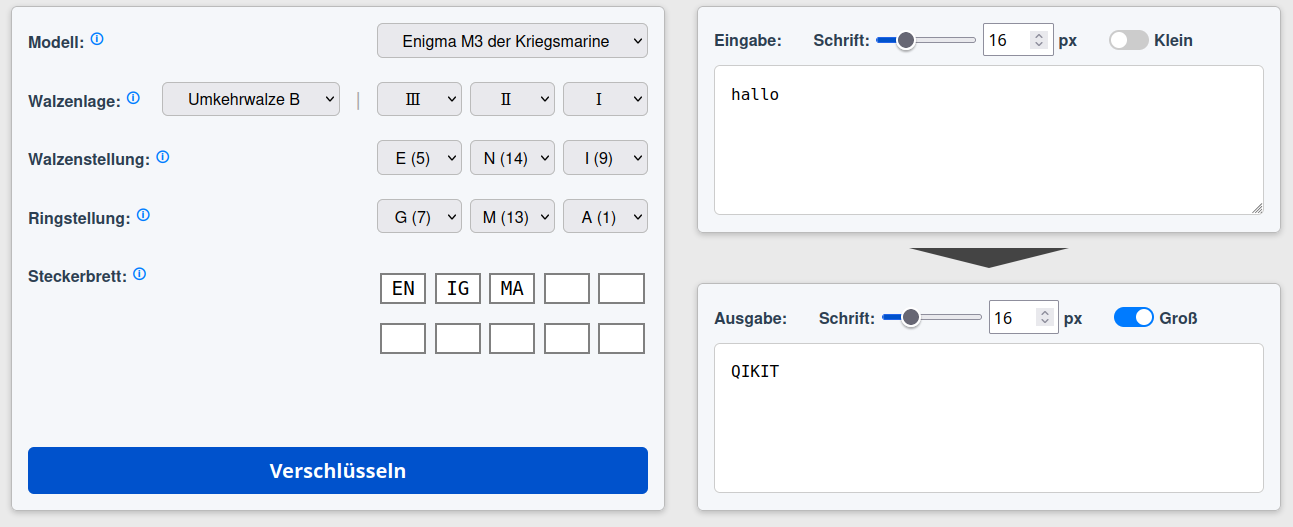
\includegraphics[width=1\textwidth]{bilder/EnigmaView.png}
	\caption{Screenshot der EnigmaView mit Beispielverschlüsselung in der eigenen Webanwendung}
	\label{fig:EnigmaView}
\end{figure}

Die Seite ermöglicht die Konfiguration einer historischen Enigma-Chiffrier\-maschine sowie die anschließende Verschlüsselung eines eingegebenen Textes über einen API-Aufruf.

\subsubsection{Benutzeroberfläche}

Die Benutzeroberfläche ist in zwei Hauptbereiche unterteilt: den linken Konfigurationsbereich und den rechten Textbereich. Im linken Bereich kann der Nutzer alle für die Enigma relevanten Parameter einstellen:

\begin{itemize}
	\item \textbf{Modell}: Auswahl des verwendeten Enigma-Modells (z.\,B. Wehrmacht M3 oder M4).
	\item \textbf{Umkehrwalze}: Festlegung der Umkehrwalze.
	\item \textbf{Walzenlage}: Auswahl und Anordnung der drei bzw. vier Walzen.
	\item \textbf{Walzenstellung}: Anfangspositionen der Walzen.
	\item \textbf{Ringstellung}: Mechanische Verschiebung der inneren Verdrahtung jeder Walze.
	\item \textbf{Steckerbrett}: Buchstabenpaare zur Substitution, einzugeben als zwei Zeichen pro Feld.
\end{itemize}

Im rechten Bereich befinden sich zwei untereinander angeordnete Textfelder. Oben wird der zu verschlüsselnde Text eingegeben, unten erscheint nach der Verschlüsselung die Ausgabe. Beide Felder sind durch das Layout optisch klar voneinander getrennt.

\paragraph{Dynamische Anpassung an das Enigma-Modell:}
Die Benutzeroberfläche passt sich, je nach ausgewähltem Enigma-Modell, automatisch an. Für die Modelle „I“ und „M3“ stehen jeweils drei Walzen zur Verfügung, wobei sich die Anzahl der auswählbaren Walzen zwischen den Modellen unterscheidet: Modell „I“ bietet fünf, Modell „M3“ hingegen acht Walzen zur Auswahl. Intern wird in beiden Fällen jedoch dieselbe Modellnummer (\lstinline|model = 3|) an die API übermittelt, da diese nur die Anzahl der eingesetzten Walzen berücksichtigt.

Beim Modell „M4“ wird zusätzlich eine vierte Walze aktiviert, was die Benutzeroberfläche um eine weitere Auswahlmöglichkeit für Walzenlage und Walzenstellung erweitert. Außerdem sind die Auswahlmöglichkeiten für die Umkehrwalze (UKW) und die vierte Walze in diesem Modus individuell konfigurierbar. In diesem Fall wird der Wert \lstinline|model = 4| an die API gesendet, um die erweiterte Konfiguration korrekt abzubilden.

Durch diese reaktive Anpassung stellt die Benutzeroberfläche sicher, dass nur gültige Konfigurationen ausgewählt werden können, was die Bedienung vereinfacht und Fehlerquellen reduziert.

\paragraph{Reaktives Texteingabefeld:}
Das Eingabefeld für den Klartext reagiert unmittelbar auf jeden Tastendruck. Über einen sogenannten Debounce-Mechanismus wird die Verarbeitung der Eingabe leicht verzögert, um eine zu hohe Anzahl von API-Anfragen zu vermeiden. So wird die Verschlüsselung dynamisch und benutzerfreundlich aktualisiert, ohne dass ein zusätzlicher Bestätigungsbutton betätigt werden muss.


\subsubsection{API-Kommunikation (/enigma)}

Die Verschlüsselung wird entweder durch Betätigung des „Verschlüsseln“-Buttons oder durch das reaktive Texteingabefeld ausgelöst. Dabei werden die aktuell gesetzten Konfigurationsparameter zusammen mit dem Eingabetext über ein POST-Request an die \lstinline|/enigma|-API gesendet.

Der Server verarbeitet die Eingabedaten mithilfe des Simulators der Enigma-Maschine und gibt den verschlüsselten Text als Antwort zurück. Diese Antwort wird anschließend direkt im Ausgabefeld der Oberfläche angezeigt.

\subsubsection{Ablauf der Verschlüsselung}

Der gesamte Ablauf erfolgt interaktiv im Browser. Die Vue-Komponente \newline \lstinline|EnigmaRequestView.vue| verwaltet dabei den Zustand der Benutzereingaben über das \lstinline|settings.enigma|-Objekt. Die Texteingabe wird zusätzlich validiert, um sicherzustellen, dass nur vom Backend unterstützte Zeichen übermittelt werden.

\subsection{Zyklometer-Seite}
\begin{figure}[H]
	\centering
	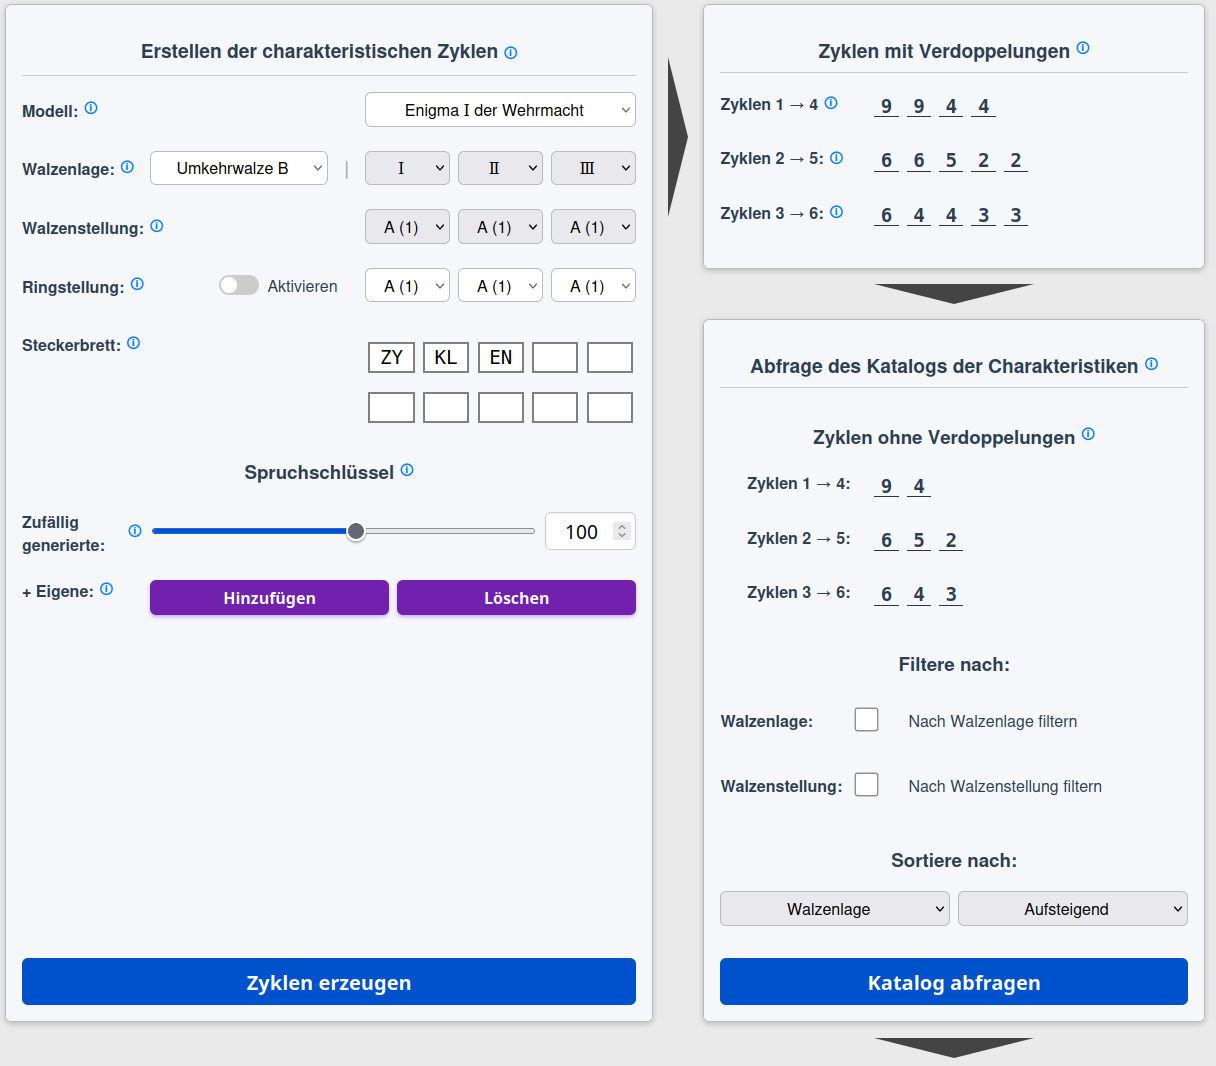
\includegraphics[width=1\textwidth]{bilder/CyclometerView_Cyclometer.png}
	\caption{Screenshot der CyclometerView mit Darstellung der charakteristischen Zyklen}
	\label{fig:CyclometerView_Cyclometer}
\end{figure}


Die Zyklometer-Seite ist in drei Hauptbereiche gegliedert und dient der Erzeugung sowie Analyse charakteristischer Zyklen der Enigma-Maschine. Sie ist unter der Route \lstinline|/cyclometer| erreichbar.


\subsubsection{Benutzeroberfläche}

Die Seite gliedert sich in folgende Bereiche:

\begin{itemize}
	\item \textbf{Linker Bereich (Eingabeformulare):}  
	Hier kann der Benutzer die Enigma-Konfiguration einstellen, inklusive Walzenlage, Walzenstellung, Ringstellung (optional aktivierbar), Steckerbrett sowie Anzahl der zufälligen und manuellen Spruchschlüssel.
	
	
	\newpage
	\item \textbf{Rechter Bereich (Ausgabe der Zyklen und Katalogabfrage):}  
	Im oberen Teil des rechten Bereichs werden die erzeugten charakteristischen Zyklen für die Permutationen 1:4, 2:5 und 3:6 angezeigt.  
	Darunter befindet sich ein Formular zur Abfrage des Katalogs mit Filter- und Sortiermöglichkeiten basierend auf Walzenlage, Walzenstellung und Zyklendaten.
	
	\item \textbf{Unterer Bereich (Tabellarische Darstellung des Katalogs):}  
	Sobald eine Katalogantwort vom Backend vorliegt, werden die Ergebnisse in einer Tabelle am unteren Seitenbereich dargestellt. Diese Tabelle zeigt detaillierte Konfigurationen mit Walzenlage, Walzenstellung sowie die jeweiligen Zyklendaten.  
	Zusätzlich sind Steuerungen zum Nachladen weiterer Einträge vorhanden, um die Übersichtlichkeit zu wahren.
\end{itemize}

	\begin{figure}[H]
	\centering
	\includegraphics[width=1\textwidth]{bilder/CyclometerView_Katalog.png}
	\caption{Screenshot der CyclometerView mit der Tabelle möglicher Enigma-Konfigurationen}
	\label{fig:CyclometerView_Katalog}
\end{figure}

Die tabellarische Darstellung der möglichen Enigma-Konfigurationen ist in Abbildung \ref{fig:CyclometerView_Katalog} zu sehen und befindet sich im unteren Bereich der Zyklometer-Seite.



\subsubsection{API-Kommunikation}

Die Kommunikation erfolgt über zwei API-Endpunkte:

\begin{itemize}
	\item \textbf{/cyclometer}: Beim Absenden des Formulars im linken Bereich werden die Enigma-Einstellungen an diesen Endpunkt gesendet. Die Antwort enthält die berechneten charakteristischen Zyklen, die im rechten oberen Bereich der Benutzeroberfläche angezeigt werden – inklusive der Zyklen mit Verdoppelungen.
	\item \textbf{/catalogue}: Die Katalogabfrage nutzt die zuvor berechneten Zyklen aus \newline \lstinline|/cyclometer| als Grundlage. Dabei werden Verdoppelungen in den Zyklenlängen herausgerechnet, indem die Anzahl ihrer Vorkommen halbiert und aufgerundet wird. Beispielsweise bleibt aus zwei Zyklen der Länge 3 ein Zyklus der Länge drei übrig. Oder bei fünf Zyklen der Länge 2 bleiben drei erhalten. Die so transformierten Zyklenlängen dienen anschließend als Filterkriterien zur Auswahl passender Enigma-Konfigurationen aus dem Katalog der Charakteristiken.
\end{itemize}


\subsubsection{Besondere Funktionen}

\begin{itemize}
	\item Die Ringstellung kann über eine Checkbox aktiviert oder deaktiviert werden und beeinflusst die Zykluserzeugung.
	\item Manuell hinzugefügte Spruchschlüssel ermöglichen individuelle Anpassungen.
	\item Sortier- und Filteroptionen für Walzenlage und Walzenstellung etc. erlauben gezielte Suchen im Katalog.
	\item Die Ergebnisliste kann in Seiten von jeweils 100 Einträgen nachgeladen werden, um Performance und Übersichtlichkeit zu optimieren.
\end{itemize}


\subsection{Benutzerführung und Darstellung}

Die Webanwendung ist so gestaltet, dass Nutzer ohne Vorkenntnisse die Verschlüsselung mit der Enigma intuitiv bedienen können. Die Bedienung des Zyklometers hingegen ist deutlich anspruchsvoller und richtet sich an Anwender mit vertieftem Verständnis der Materie. Um die Nutzung zu erleichtern, sind zahlreiche Tooltips integriert, die wichtige Hinweise und Erklärungen liefern.

Darüber hinaus steht eine separate Seite mit einer ausführlichen Bedienungsanleitung zur Verfügung.

Die klare Aufteilung in Eingabe-, Ausgabebereiche und Ergebnislisten unterstützt eine logische Abfolge der Arbeitsschritte. Hinweise und Validierungen erleichtern die korrekte Eingabe kryptografischer Parameter und verhindern Fehler frühzeitig.

Die interaktive Darstellung der Zyklen und der Enigma-Konfigurationen erfolgt in übersichtlichen Tabellen und visualisierten Komponenten, die auf Benutzeraktionen reagieren. Zudem werden Lade- und Bearbeitungszustände visuell kommuniziert, um Transparenz im Ablauf zu schaffen.


\newpage
\section{Inbetriebnahme und Nutzung der Quellcodebasis}
\label{sec:nutzung}

Der vollständige Quellcode dieser Arbeit ist in vier öffentlich zugänglichen Repositories auf \lstinline|GitHub| verfügbar. Jede Komponente wird mit einer eigenen \lstinline|README.md|-Datei dokumentiert, die alle relevanten Installations- und Konfigurationshinweise enthält. Neben den bereits beschriebenen Projekten steht auch das Repository der Bachelorarbeit selbst zur Verfügung, welches die gesamte Dokumentation und die Codebasis bündelt \autocite{bibblecode2025enigmazyklometer}.

In diesem Kapitel wird die Vorgehensweise zur Installation, Konfiguration und Ausführung der Softwarekomponenten beschrieben.


\subsection{Quellcodeübersicht}

\begin{itemize}

	
	\item \textbf{Native Enigma-Simulation}  
	\newline \lstinline|https://github.com/UPEV1sion/Enigma/tree/server|
	
	Beinhaltet den Quellcode der Enigma-Simulation in \lstinline|C| sowie das Buildsystem zur Erzeugung der \lstinline|libenigma.so|.
	
	\item \textbf{Backend REST API}  
	\newline \lstinline|https://github.com/UPEV1sion/Enigma-API|  
	
	Enthält die Spring Boot Anwendung, welche über die \newline\lstinline|FFM API API| mit dem nativen C-Backend kommuniziert.
	
	\item \textbf{Webfrontend (Vue 3)}  
	\newline \lstinline|https://github.com/Bibble-code/EnigmaSite|
	
	Implementiert das interaktive Interface zur Enigma und zum Zyklometer. Die Anwendung kann lokal über \lstinline|npm| gestartet oder als statische Website gebaut werden.
\end{itemize}

\newpage
\subsection*{Installation und Start}

Für die vollständige Inbetriebnahme sind drei separat zu konfigurierende Komponenten erforderlich: die native Bibliothek, das Java-Backend und das Webfrontend. Die folgende Übersicht beschreibt die zentralen Schritte.

\subsubsection*{1. Native Bibliothek (\texttt{libenigma.so})}

Die Enigma-Simulation ist in \lstinline|C| implementiert und muss manuell aus dem separaten Repository \lstinline|Enigma/tree/server| kompiliert werden.  
Dabei ist wie folgt vorzugehen:

\begin{itemize}
	\item Repository klonen und gemäß der dortigen \lstinline|README.md| einrichten.
	\item \lstinline|cmake| und \lstinline|make| ausführen, um die Datei \lstinline|libenigma.so| zu erzeugen.
	\item Die erzeugte \lstinline|.so|-Datei nach \lstinline|src/main/enigma_c/| im Backend-Projekt kopieren.
\end{itemize}

\textit{Hinweis:} Die Datei wird absichtlich nicht versioniert und muss lokal erzeugt werden.  
Dabei ist darauf zu achten, dass die Kompilierung \textbf{für das Zielsystem} erfolgt (z.\,B. passende Architektur und \lstinline|glibc|-Version), da unter Linux systemnahe Inkompatibilitäten auftreten können — selbst zwischen gängigen Distributionen wie Ubuntu und Arch Linux.

\subsubsection*{2. Backend (Spring Boot)}

Das Backend ist eine Java-Anwendung, die über die FFM API auf die native Bibliothek zugreift. Zur Vorbereitung:

\begin{itemize}
	\item \lstinline|Java 22+| und \lstinline|Maven 3.9+| installieren.
	\item Datenbank initialisieren:
	\begin{itemize}
		\item PostgreSQL 17+ installieren.
		\item Datenbank und Benutzer gemäß \lstinline|application.properties| anlegen.
		\item SQL-Dump entpacken: \lstinline|unzip db/init.sql.zip|
		\item Dump importieren:  
		\lstinline|psql -U <user> -d <datenbankname> < init.sql|
	\end{itemize}
	\item Weitere Details enthält \lstinline|db/README.md|.
	\item Backend starten:
	
	\lstinline|mvn clean install|  
	\lstinline|java --enable-native-access=ALL-UNNAMED -jar target/Enigma_API.jar|
\end{itemize}

\subsubsection*{3. Frontend (Vue 3)}

Die grafische Benutzeroberfläche basiert auf Vue 3 und kommuniziert über HTTP mit dem Backend.

\begin{itemize}
	\item \lstinline|Node.js| und \lstinline|npm| installieren.
	\item Abhängigkeiten mit \lstinline|npm install| installieren.
	\item Start im Entwicklungsmodus: \lstinline|npm run serve|
	\item Optional: \lstinline|npm run build| für Produktionsbuild
\end{itemize}




\subsection{Veröffentlichte Anwendung}

Die im Rahmen dieser Arbeit entwickelte Webanwendung ist öffentlich zugänglich unter:  
\lstinline|https://enigma-zyklometer.rwu.de|

\subsection{Detaillierte Anleitungen in den README-Dateien}

Die vollständigen Anleitungen zur Installation, Konfiguration und Nutzung der einzelnen Komponenten befinden sich jeweils in den \lstinline|README.md|-Dateien der zugehörigen Repositories.  
Sie enthalten unter anderem Hinweise zur Datenbankeinrichtung, zu Lizenzinformationen sowie zu Build- und Startprozessen.  





\newpage
\section{Evaluation und Reflexion}

\subsection{Selbstständige Konzeption und Zielerreichung}

Die Aufgabe, eine bestehende C-Implementierung der Enigma-Maschine als Webanwendung öffentlich zugänglich zu machen, bot großen gestalterischen Spielraum und stellte dadurch hohe Anforderungen an die eigenständige Konzeption und Umsetzung. Rückblickend wurde das übergeordnete Ziel erreicht: Die Anwendung ist online verfügbar, verbindet moderne Webtechnologien mit systemnaher Programmierung und erfüllt sowohl funktionale als auch technische Anforderungen.

\subsection{Herausforderungen in der technischen Umsetzung}

Die Anbindung der bestehenden C-Implementierung der Enigma-Maschine an die Java-basierte Webarchitektur stellte erhebliche technische Herausforderungen dar. Zwar gestaltete sich die Umsetzung der FFM API zunächst als schwierig und zeitaufwändig, dennoch erwies sich der Einsatz von FFM letztlich als die richtige Entscheidung. Die FFM API ermöglichte eine stabile Schnittstelle, die den Datenaustausch zwischen C und Java zuverlässig realisierte.

Auch die Anbindung der PostgreSQL-Datenbank erwies sich als anspruchsvoll. Die Entwicklung performanter und komplexer Abfragen im Java-Backend erforderte umfangreiche Optimierungen und ein tiefgehendes Verständnis der Datenbank- und Framework-Mechanismen. Besonders die Performanceoptimierung des Katalogsystems erwies sich als deutlich aufwändiger als zunächst erwartet und erforderte wiederholte Anpassungen, um eine flüssige Benutzererfahrung sicherzustellen.


\subsection{Komplexität und Schnittstellenproblematik}

Das Projekt erforderte die Koordination eines umfangreichen Technologie-Stacks, von C über Java mit Spring Boot und PostgreSQL bis zum Vue3-Frontend. Änderungen an einer Komponente hatten häufig Auswirkungen auf andere Bereiche, was die Komplexität erhöhte und die Fehleranfälligkeit steigerte.


\newpage
\section{Fazit und Ausblick}

Die Arbeit zeigt die erfolgreiche Umsetzung einer komplexen technischen Aufgabe: Die Überführung einer systemnahen C\hyp{}Implementierung der Enigma-Maschine und insbesondere des Zyklometers in eine moderne, öffentlich zugängliche Webanwendung.

Dabei ist es gelungen, erstmals eine funktionierende Simulation des Zyklometers online zur Verfügung zu stellen. So kann die Funktionsweise des Zyklometers besser verstanden und die Analyse der Zyklen praktisch nachvollzogen werden.

Für die Zukunft bieten sich ein paar größere Erweiterungen an, die das Potenzial der Anwendung deutlich steigern könnten:

\begin{itemize}
	\item \textbf{Aufteilung der Zyklometer-Abfrage in zwei Stufen:}  
	Die derzeitige Zyklometer-Abfrage kombiniert derzeit zwei Funktionalitäten: Die Verschlüsselung der Spruchschlüssel und die Generierung der Zyklen aus diesen. Eine Aufteilung könnte wie folgt aussehen:
	
	Die erste Stufe erzeugt aus unverschlüsselten Spruchschlüsseln verschlüsselte Spruchschlüssel basierend auf einer Enigma-Konfiguration. In der zweiten Stufe werden anschließend aus diesen verschlüsselten Schlüsseln die charakteristischen Zyklen gebildet. Diese Zweistufigkeit würde die Simulation der sogenannten „deutschen“ und „polnischen“ Seite des Zyklometers realistischer abbilden und die Analyse präzisieren.
	
	\item \textbf{Erweiterung um die Entzifferung der Spruchschlüssel:}  
	Derzeit können mit dem Zyklometer nur Walzenlage und Walzenstellung bestimmt werden, nicht jedoch die Steckerbrett-Verbindungen. Eine zukünftige Erweiterung könnte eine neue Abfrage implementieren, die eine Entzifferung der Steckerbrett-Konfiguration erlaubt.
	
	\item \textbf{Integration eines mit dem Spruchschlüssel verschlüsselten Texts:}  
	Zusätzlich zum verschlüsselten Spruchschlüssel könnte ein kurzer Nachrichtentext übermittelt werden, der mit dem jeweiligen Spruchschlüssel verschlüsselt wird. Nach Rekonstruktion sämtlicher Enigma-Parameter (einschließlich Steckerbrett) könnte zunächst der Spruchschlüssel und anschließend mit diesem der Text entschlüsselt werden. Dies würde eine realitätsnähere Simulation des vollständigen kryptographischen Ablaufs ermöglichen.
	
	\item \textbf{Skalierbarkeit und Deployment:}  
	Bisher wurde auf eine containerisierte Bereitstellung (z.\,B. mit Docker) verzichtet. Eine solche Maßnahme könnte die Skalierbarkeit und Performance der Webanwendung verbessern und den Betrieb vereinfachen.
\end{itemize}

Diese Weiterentwicklungen würden nicht nur die Funktionalität vertiefen, sondern auch den praktischen Nutzen der Anwendung steigern.


%
%\newpage
%\section*{Glossar}
%\addcontentsline{toc}{section}{Glossar}
%
%% Frontend-Technologien
%\subsection*{Frontend-Technologien}
%TODO Prinzip der klaren Verantwortlichkeit.
%\begin{description}
%	\item[Vue.js:] Ein progressives JavaScript-Framework zur Erstellung interaktiver Benutzeroberflächen. Es ähnelt AngularJS und React, ist aber besonders leichtgewichtig und flexibel.
%	
%	\item[Vue 3:] Die aktuelle Hauptversion von Vue.js, die neue Features wie die Composition API für bessere Code-Organisation und höhere Leistung bietet.
%	
%	\item[Vue CLI:] Ein Kommandozeilen-Werkzeug zum schnellen Erstellen und Verwalten von Vue-Projekten mit integrierten Build-Tools und Plugins.
%	
%	\item[DOM:] Das Document Object Model ist eine standardisierte, baumartige Darstellung von HTML- und XML-Dokumenten, die es Skriptsprachen wie JavaScript ermöglicht, Inhalte, Struktur und Stil einer Webseite dynamisch zu verändern.
%		
%	\item[Framework:] 
%	Eine wiederverwendbare Softwarestruktur, die als Gerüst für die Entwicklung von Anwendungen dient. 
%	Frameworks stellen vorgefertigte Funktionen und Konventionen bereit, um typische Programmieraufgaben zu vereinfachen und zu standardisieren. 
%	Beispiele sind \emph{Spring Boot} für Java oder \emph{Vue.js} für das Web-Frontend.
%	
%	\item[Single-File Component (SFC):] Dateien, die Template, Logik und Styles in einer einzigen .vue-Datei bündeln und so modularen und übersichtlichen Code ermöglichen.
%	
%	\item[Composition API:] Ein modernes Programmiermodell in Vue 3 zur besseren Strukturierung von Komponentenlogik, besonders nützlich für komplexe Anwendungen.
%	
%	\item[Single-Page Application (SPA):] Webanwendungen, die in einer einzelnen HTML-Seite laufen und Inhalte dynamisch nachladen, um schnelle und flüssige Nutzererlebnisse zu ermöglichen.
%	
%	\item[Axios:] Eine JavaScript-Bibliothek zum einfachen Senden von HTTP-Anfragen, besonders für die Kommunikation mit REST-APIs.
%	
%	\item[CORS (Cross-Origin Resource Sharing):] Ein Sicherheitsmechanismus, der steuert, welche Ressourcen von einer Webdomain aus auf eine andere zugreifen dürfen.
%	
%	\item[Preflight-Anfrage:] Eine automatische OPTIONS-Anfrage des Browsers zur Überprüfung von CORS-Richtlinien vor der eigentlichen HTTP-Anfrage.
%	
%	\item[History API:] Browser-API zur Manipulation des Verlaufs und der URL, wichtig für Navigation in SPAs ohne Seitenreload.
%\end{description}
%
%% Backend-Technologien \& Java
%\subsection*{Backend-Technologien \& Java}
%
%\begin{description}
%	\item[Backend:] Der Teil einer Anwendung, der serverseitig Daten verarbeitet, Logik ausführt und Schnittstellen zu Datenbanken bereitstellt.
%	
%	\item[API (Application Programming Interface):]
%	Eine Schnittstelle, die es ermöglicht, dass verschiedene Softwarekomponenten miteinander kommunizieren. 
%	APIs definieren, wie Funktionen, Daten und Dienste von einem Programm für andere Programme zugänglich gemacht werden. 
%	Beispiele in diesem Projekt sind die \emph{FFM API} zur Anbindung nativer Funktionen und die \emph{Enigma-API} als REST-Schnittstelle zur Enigma-Verschlüsselung.
%	
%	
%	  \item[Spring Boot:] 
%	Ein Framework zur Entwicklung von Java-Anwendungen, das auf dem Spring-Framework aufbaut.  
%	Es ermöglicht durch Konventionen und automatische Konfiguration eine schnelle Einrichtung von produktionsreifen Webanwendungen.  
%	Spring Boot unterstützt die Entwicklung von REST-APIs, Validierung (z.\,B. mit \lstinline|javax.validation|) sowie Dependency Injection und bietet umfangreiche Middleware-Integration.
%
%	
%	
%	\item[REST (Representational State Transfer):]
%	Ein Architekturstil für Webservices, der auf HTTP-Methoden (GET, POST, PUT, DELETE) basiert. 
%	REST definiert Prinzipien wie zustandslose Kommunikation, klare Ressourcennamen (URLs) und standardisierte Operationen. 
%	APIs, die diese Prinzipien befolgen, werden als \emph{RESTful} bezeichnet und ermöglichen einfache, skalierbare und leicht verständliche Schnittstellen.
%	
%	
%	\item[RESTful HTTP-API:] Eine Web-API, welche die Prinzipien von REST nutzt, um Ressourcen über HTTP-Methoden zugänglich zu machen.
%	
%	\item[DTO (Data Transfer Object):] Einfache Datenstruktur zur Übertragung von Daten zwischen verschiedenen Schichten einer Anwendung, z.\,B.\ zwischen Controller und Service.
%	
%	
%	\item[ResponseEntity:] Klasse zur flexiblen Modellierung von HTTP-Antworten, inklusive Statuscode und Headern.
%	
%	\item[Service-Schicht:] Softwarearchitektur-Schicht, die Geschäftslogik kapselt und von Controllern genutzt wird.
%	
%	\item[JDBC (Java Database Connectivity):] Standard-API in Java zur Kommunikation mit relationalen Datenbanken.
%	
%	\item[Hibernate:] Java-Framework für Objekt-Relationale Abbildung (ORM), das SQL-Komplexität reduziert.
%	
%	\item[Java Foreign Function \& Memory API (FFM API):] 
%	Eine moderne Java-API zur effizienten und sicheren Anbindung nativer Bibliotheken (z.\,B. in C). 
%	Sie ermöglicht direkten Zugriff auf native Funktionen und Speicher, als Nachfolger des älteren JNI-Mechanismus, mit einfacherem und performanterem Code.
%	
%	
%	\item[Java Native Interface (JNI):] Ältere Schnittstelle zum Aufruf nativer Bibliotheken aus Java, komplexer als FFM API.
%	
%	\item[Native Funktion:] Funktion, die außerhalb der Java Virtual Machine (JVM) in einer anderen Programmiersprache wie C oder C++ implementiert ist und über Schnittstellen wie JNI oder die Foreign Function \& Memory API (FFM API) von Java aufgerufen wird.
%	
%\end{description}
%
%% Datenbanken \& Indizes
%\subsection*{Datenbanken \& Indizes}
%
%\begin{description}
%	\item[PostgreSQL:] Leistungsstarkes, objektrelationales Open-Source-Datenbank\hyp{}system mit umfangreichen Managementfunktionen.
%	
%	
%	\item[Primärschlüssel:] 
%	Ein eindeutiges Attribut oder eine Attributkombination, die jeden Datensatz in einer Tabelle eindeutig identifiziert. 
%	Primärschlüssel sind fundamental für Datenintegrität und die Herstellung von Beziehungen in relationalen Datenbanken.  Besteht der Primärschlüssel aus mehreren Attributen, so spricht man von einem zusammengesetzten Primärschlüssel.
%	
%	\item[Fremdschlüssel:] 
%	Ein Attribut, das auf einen Primärschlüssel einer anderen Tabelle verweist und somit eine Beziehung zwischen Tabellen definiert. 
%	Fremdschlüssel sorgen für referenzielle Integrität und verhindern inkonsistente Daten.
%	
%	
%	\item[Normalisierung:] 
%	Ein Verfahren zur Strukturierung von Datenbanken, das Redundanzen vermeidet und die Datenintegrität durch die Einhaltung von Normalformen (z.\,B. dritte Normalform, 3NF) sicherstellt. 
%	Normalisierung verbessert die Wartbarkeit und Konsistenz der Daten.
%	
%	
%	\item[GIN-Index (Generalized Inverted Index):] 
%	Ein spezieller Index in PostgreSQL, der schnelle Volltextsuche und Abfragen auf komplexen Datentypen wie Arrays und JSONB ermöglicht. 
%	Er optimiert Suchanfragen durch Invertierung der Datenstruktur.
%
%	
%	\item[Containment Operator (@>|):] Operator zur Abfrage, ob ein Array oder JSON ein bestimmtes Element enthält.
%	
%	\item[Pagination:] 
%	Die Unterteilung großer Datenmengen in überschaubare Seiten (Pages) zur Verbesserung der Performance und Nutzerfreundlichkeit. 
%	Pagination reduziert die Netzwerklast und die Ladezeiten beim Abrufen von Datensätzen aus der Datenbank.
%	
%	\item[Caching:] Zwischenspeicherung von Daten zur Beschleunigung von Anfragen.
%\end{description}
%
%% Server \& Infrastruktur
%\subsection*{Server \& Infrastruktur}
%
%\begin{description}
%	\item[nginx:] Beliebter, performanter Webserver und Reverse-Proxy.
%	
%	\item[Reverse-Proxy:] Server, der Anfragen an Backend-Server weiterleitet, oft für Lastverteilung und Sicherheit genutzt.
%	
%	\item[Reverse-Proxy-Konfiguration:] Einstellung eines Reverse-Proxys zur Steuerung der Weiterleitung und Sicherheit.
%	
%	\item[Proxy-Konfiguration:] Allgemeine Servereinstellungen für Vermittlerfunktionen.
%	
%	\item[systemd-Dienst:] Linux-Manager für Hintergrundprozesse (Dienste).
%	
%	\item[HTTP-Kompression:] 
%	Verfahren zur Reduktion der Größe von HTTP-Antworten zur Beschleunigung der Datenübertragung.
%	
%	\item[Caching:] 
%	Zwischenspeicherung häufig genutzter Daten, um Ladezeiten und Serverlast zu verringern.
%	
%\end{description}
%
%% Speicher \& Programmierung
%\subsection*{Speicher \& Programmierung}
%
%\begin{description}
%	\item[MemorySegment:] Speicherbereich in der Java FFM API für sicheren Zugriff auf nativen Speicher.
%	
%	\item[MethodHandle:] Java-Objekt zur dynamischen Methodenreferenzierung.
%	
%	\item[FunctionDescriptor:] Beschreibung der Signatur nativer Funktionen für die FFM API.
%	
%	\item[Speicher-Layout (MemoryLayout):] Anordnung von Daten im Speicher für Kompatibilität mit nativen Bibliotheken.
%	
%	\item[Speicher-Alignment:] Ausrichtung von Daten im Speicher für effizienten Zugriff.
%	
%	\item[Padding:] Speicherauffüllung, um Alignment sicherzustellen.
%	
%	\item[Pointer:] Speicheradresse, die auf Daten oder Funktionen zeigt.
%	
%	\item[ASCII-kodiert:] Standardzeichensatz mit 128 Zeichen, genutzt für einfache Textdarstellung.
%	
%	\item[Nullterminiertes char**-Array:] In C ein Array von Zeichenketten, das durch ein Null-Zeichen abgeschlossen ist.
%\end{description}
%
%% Sonstiges
%\subsection*{Sonstiges}
%
%\begin{description}
%	\item[Permutationen:] Alle möglichen Anordnungen einer Menge von Elementen.
%\end{description}
%\newpage



%\printglossary[type=frontend,title={Frontend-Technologien}]
%\printglossary[type=backend,title={Backend-Technologien und Java}]
%\printglossary[type=db,title={Datenbanken und Indizes}]
%\printglossary[type=server,title={Server und Infrastruktur}]
%\printglossary[type=misc,title={Speichertechnologien}]

\glsnogroupskiptrue
\renewcommand*{\glossaryentrynumbers}[1]{}

\clearpage
\phantomsection
\addcontentsline{toc}{section}{Glossar}
\section*{Glossar}
\printglossary[type=frontend, title={Frontend-Technologien}, toctitle={}]
\printglossary[type=backend, title={Backend-Technologien und Java}, toctitle={}]
\printglossary[type=db, title={Datenbanken und Indizes}, toctitle={}]
\printglossary[type=server, title={Server und Infrastruktur}, toctitle={}]
\printglossary[type=misc, title={Speichertechnologien}, toctitle={}]



\newpage
\printbibliography[heading=bibintoc]
\end{document}

